\documentclass[journal,10pt]{IEEEtran}
\usepackage[utf8]{inputenc}
\usepackage[T1]{fontenc}
\usepackage{algorithm}
\usepackage{algorithmic}
\usepackage[linktoc=all, bookmarksdepth=3, pdfstartview=FitH]{hyperref}
\hypersetup{colorlinks=true, linkcolor=blue, filecolor=magenta, urlcolor=cyan}
\urlstyle{same}
\usepackage{amsmath}
\usepackage{amsfonts}
\usepackage{amssymb}
\usepackage{graphicx}
\usepackage[export]{adjustbox}
\usepackage[dvipsnames]{xcolor}
\usepackage{float}
\usepackage{placeins}
\usepackage{caption}
\captionsetup[figure]{name=Fig.}
\usepackage{booktabs}
\usepackage{multirow}
\usepackage{subcaption}
\usepackage{url}
\usepackage{cite}

\graphicspath{ {./} }

\title{Uncertainty-regularized offline reinforcement learning matches offline-to-online fine-tuning for bus holding control: A SUMO benchmark}

\author{Zhang~Yifan, and~Liang~Zheng%
\thanks{Z. Yifan and L. Zheng are with the School, Central South University, Changsha, China. E-mail: \href{mailto:erzhu419@gmail.com}{erzhu419@gmail.com}, \href{mailto:204201048@csu.edu.cn}{204201048@csu.edu.cn}, \href{mailto:zhengliang@csu.edu.cn}{zhengliang@csu.edu.cn}.}%
\thanks{Code is available at \url{https://github.com/erzhu419/offline-sumo}.}}

\begin{document}
\maketitle

\begin{abstract}
Bus holding control requires reinforcement learning (RL) policies that learn from operational logs without expensive online interaction. We benchmark four families of methods on a Changsha-calibrated SUMO microscopic simulation of a real bus network (389 buses, 12 lines, 353 stops), using a single policy that controls all 12 lines simultaneously through line and bus embeddings, trained from 3.1 million offline transitions recorded under a heuristic controller across the full network. Our comparison includes (i) pure offline methods: behavior cloning, an H2O+ advantage-weighted regression baseline, and conservative $Q$-learning (CQL)~\cite{kumar2020conservative}; (ii) pure online soft actor-critic (SAC); and (iii) two state-of-the-art offline-to-online approaches, WSRL~\cite{zhou2024efficient} and RLPD~\cite{ball2023efficient}. We also introduce RE-SAC offline, a pure offline algorithm built as an additive stack: an offline actor-critic with a behavior-cloning anchor, a 10-head $Q$-ensemble, and a lower-confidence-bound (LCB) pessimism term; our ablation shows that the offline + ensemble + LCB stack is what produces the headline result, with no single component being uniquely responsible (an $L_1$ weight-norm penalty is harmless on Best and slightly hurts Final, so the canonical recipe drops it). We also introduce a rigorous post-hoc evaluation protocol that re-evaluates every saved checkpoint on 10 fresh SUMO episodes, and show that the ``best'' checkpoint metric commonly reported in offline-to-online RL work can overstate performance by 10--25\% on the weakest baselines relative to this protocol. Across 630 post-hoc-evaluated checkpoints (5 seeds for the four-way main comparison and 3 seeds for the remaining baselines and ablation cells; per-method counts in Table~\ref{tab:ckpt_inventory}), we find: (1) standard offline baselines overfit---behavior cloning and the H2O+ offline variant both peak early then degrade to $-9439$ and $-9482$ respectively by the end of training, while the canonical conservative offline RL baseline CQL is competitive on best return ($-4992$) but degrades to $-5942$ at convergence, exhibiting the same overfitting pattern at smaller magnitude; (2) offline-to-online methods (WSRL, RLPD, and their architecture-matched 10-head variants) attain stable final returns in the band $-4634$ to $-4965$; (3) online SAC attains only $-7052$ and exhibits value-function instability under extended training; and (4) RE-SAC offline achieves $-4184 \pm 157$ (best) and $-4550 \pm 213$ (final, 5 seeds, 95\% CI $\pm 86$; seed-level $\sigma$ uses ddof=0 to match figures), without any online environment interaction. A preliminary single-seed extended-budget experiment (online SAC for 600 epochs) suggests this gap is not closed by simply training online SAC longer, though a multi-seed confirmation is left to future work. We release all code, data, and evaluated checkpoints.
\end{abstract}

\begin{IEEEkeywords}
Deep reinforcement learning, offline reinforcement learning, offline-to-online reinforcement learning, bus holding control, multi-line transit, ensemble $Q$-learning, lower-confidence-bound pessimism, SUMO.
\end{IEEEkeywords}

\section{Introduction}
\label{sec:intro}

Public-transit bus holding---delaying a bus at a stop to restore headway uniformity---is a canonical real-world control problem plagued by \textit{bus bunching}: small perturbations propagate and cluster buses, degrading service quality~\cite{daganzo2009headway,bartholdi2012self}. Reinforcement learning has been applied to bus holding~\cite{alesiani2018reinforcement,wang2020holding}, but deploying on-policy training on a real bus line is operationally risky and slow. Offline RL and offline-to-online fine-tuning are natural fits: a fleet of buses generates operational logs continuously, and new policies can be trained without incurring the cost of exploratory interaction~\cite{levine2020offline}.

The offline-to-online literature offers two dominant recipes. Warm-start RL (WSRL)~\cite{zhou2024efficient} pre-trains a policy on offline data and discards the data for online fine-tuning, arguing that extended use of offline data creates distributional mismatch. RLPD~\cite{ball2023efficient} initializes a policy from scratch and samples half-and-half from offline and online buffers throughout training, relying on simple data mixing. Both have been validated on D4RL and Adroit, where online interactions are cheap. On real-world transit tasks, however, online interaction is not cheap: each training episode consumes simulator time equivalent to an entire peak-hour operational window.

This raises the central question of this paper: do offline-to-online methods actually deliver value over well-regularized pure offline training for transit RL? Our answer, framed conservatively, is: \emph{not under the comparisons we tested}. On a production-scale SUMO simulation of a real bus network, we show that a pure offline algorithm with proper uncertainty regularization---which we call RE-SAC offline---matches or directionally exceeds all tested offline-to-online methods while requiring zero online rollouts. The standard twin-$Q$ variants of WSRL and RLPD are clearly outperformed; the architecture-matched 10-head WSRL-E10 variant narrows the gap considerably and is statistically tied with RE-SAC at the 95\% level on Best (Sec.~\ref{sec:results}); RLPD-E10 remains significantly behind. In other words, the present evidence does not support a reliable advantage for offline-to-online fine-tuning over a strong pure-offline learner in this setting, but it also does not categorically rule out a closely-matched 10-head warm-start baseline. The main empirical lesson is that an offline actor-critic + ensemble + LCB \emph{stack} is a strong zero-online baseline worth considering before the engineering overhead of staged offline-to-online fine-tuning, not that offline RL universally dominates.

Our contributions are summarized as follows:
\begin{itemize}
  \item \textbf{Benchmark.} A reproducible SUMO benchmark for offline and offline-to-online RL on a realistic whole-network bus-holding task. A single categorical-embedding policy controls all 12 lines (389 buses, 353 stops) simultaneously, trained on 3.1 million offline transitions generated by a heuristic controller across the full Changsha-calibrated microsimulation ($\sim$98{,}000 social-vehicle trips and 15{,}079 passengers per 2.5-hour episode).
  \item \textbf{Algorithm.} RE-SAC offline, a pure offline algorithm built as a stack of three additive components: an offline actor-critic with a behavior-cloning anchor (already strong on its own), a 10-head $Q$-ensemble (adds $\Delta\!\approx\!141$ Best return, $p\!=\!0.009$), and a lower-confidence-bound (LCB) pessimism term (adds another $\Delta\!\approx\!112$ Best, $p\!=\!0.023$). An $L_1$ weight-norm penalty is harmless on Best but slightly hurts Final stability, so the canonical recipe is offline actor-critic + ensemble + LCB.
  \item \textbf{Evaluation protocol.} A rigorous post-hoc evaluation protocol: every saved checkpoint is re-evaluated on 10 SUMO episodes across three or five seeds (630 checkpoints total including baselines, intermediate curves, and ablations; per-cell counts in Table~\ref{tab:ckpt_inventory}), exposing that during-training ``best'' metrics reported by existing offline-to-online work can overstate performance by 10--25\% on the weakest baselines.
  \item \textbf{Extended budget study (single seed, indicative).} A preliminary single-seed extended online SAC training study (600 epochs) suggests that simply doubling the online SAC budget does not reliably close the gap to RE-SAC offline: SAC plateaus around $-6500$ and exhibits transient peaks from value-function instability rather than steady convergence. A multi-seed replication is left to future work.
\end{itemize}

\section{Related work}
\label{sec:related}

\subsection{Offline reinforcement learning}
Offline RL learns from fixed logs without online interaction, addressing extrapolation error via conservatism~\cite{kumar2020conservative}, implicit value regression~\cite{kostrikov2022offline}, or ensemble pessimism. Our RE-SAC method draws on the randomized ensembled double $Q$-learning (REDQ) architecture~\cite{chen2021randomized} and the robust offline RL of Yang et al.~\cite{yang2022rorl}, who use $Q$-function ensembles to enforce pessimism through lower-confidence bounds.

\subsection{Offline-to-online fine-tuning}
WSRL~\cite{zhou2024efficient} argues that retaining offline data during online fine-tuning causes the replay buffer to drift and degrade, so the offline data should be discarded after warm-start. RLPD~\cite{ball2023efficient} takes the opposite view: sample 50/50 from offline and online data throughout training; the offline data stabilizes $Q$-function updates. Cal-QL~\cite{nakamoto2023calql} proposes calibration on top of conservative $Q$-learning for offline-to-online transfer. H2O/H2O+~\cite{niu2022trust} tackles sim-to-real by learning a dynamics discriminator between simulator and real logs; we include its offline-only mode (advantage-weighted-regression-based) as the H2O+ offline baseline.

\subsection{Bus holding control}
Headway-based holding~\cite{daganzo2009headway,bartholdi2012self} is the classical control-theoretic baseline. Early RL approaches~\cite{alesiani2018reinforcement,wang2020holding} train tabular or simple deep policies on analytical simulators without real data. Our benchmark uses a microsimulation calibrated against real passenger origin-destination matrices and vehicle routes.

\section{Problem setup}
\label{sec:setup}

\subsection{Simulator: SUMO microscopic traffic simulation}
\label{sec:sumo}

\paragraph{SUMO overview.} Eclipse SUMO (simulation of urban mobility) version 1.25~\cite{lopez2018microscopic} is an open-source, space-continuous, time-discrete microscopic traffic simulator. Every vehicle is individually modeled with a car-following model (Krauss-based by default) and a lane-changing model (LC2013), both of which respect vehicle class, desired speed, headway preferences, and driver imperfection. Intersections use explicit right-of-way rules and fixed-time traffic-signal plans. We drive the simulator through \texttt{libsumo}, an in-process C++ application programming interface that bypasses the TraCI socket protocol and is roughly 10$\times$ faster than TraCI for the dense-observation regime we need. The simulator step length is set to 0.5\,s.

\paragraph{Changsha bus network.} Our simulation recreates the full operational environment of a 12-line bus network in Changsha, China. The network was calibrated against the real city topology and real passenger origin-destination survey data. Its size and composition are summarized in Table~\ref{tab:sumo_stats} and its spatial layout is shown in Fig.~\ref{fig:network}. Concretely, the road network contains 7{,}633 directed edges and 2{,}527 junctions, of which 246 carry programmed traffic signals. Buses, social vehicles, and pedestrians are all first-class agents: bus vehicles (\texttt{vClass=bus}, 50-passenger capacity, 4\,s per-stop boarding time) share road edges with $\sim$98{,}000 social vehicle trips across two scenario files ($c_1$: dense weekday traffic, 61{,}044 trips; $c_2$: lighter weekday traffic with added bypass routes, 37{,}644 trips), and service 15{,}079 simulated passengers whose trip plans are drawn from origin-destination matrices calibrated against transit card data (14{,}211 regular workday trips plus 868 inter-line transfer trips).

\begin{figure}[!t]
  \centering
  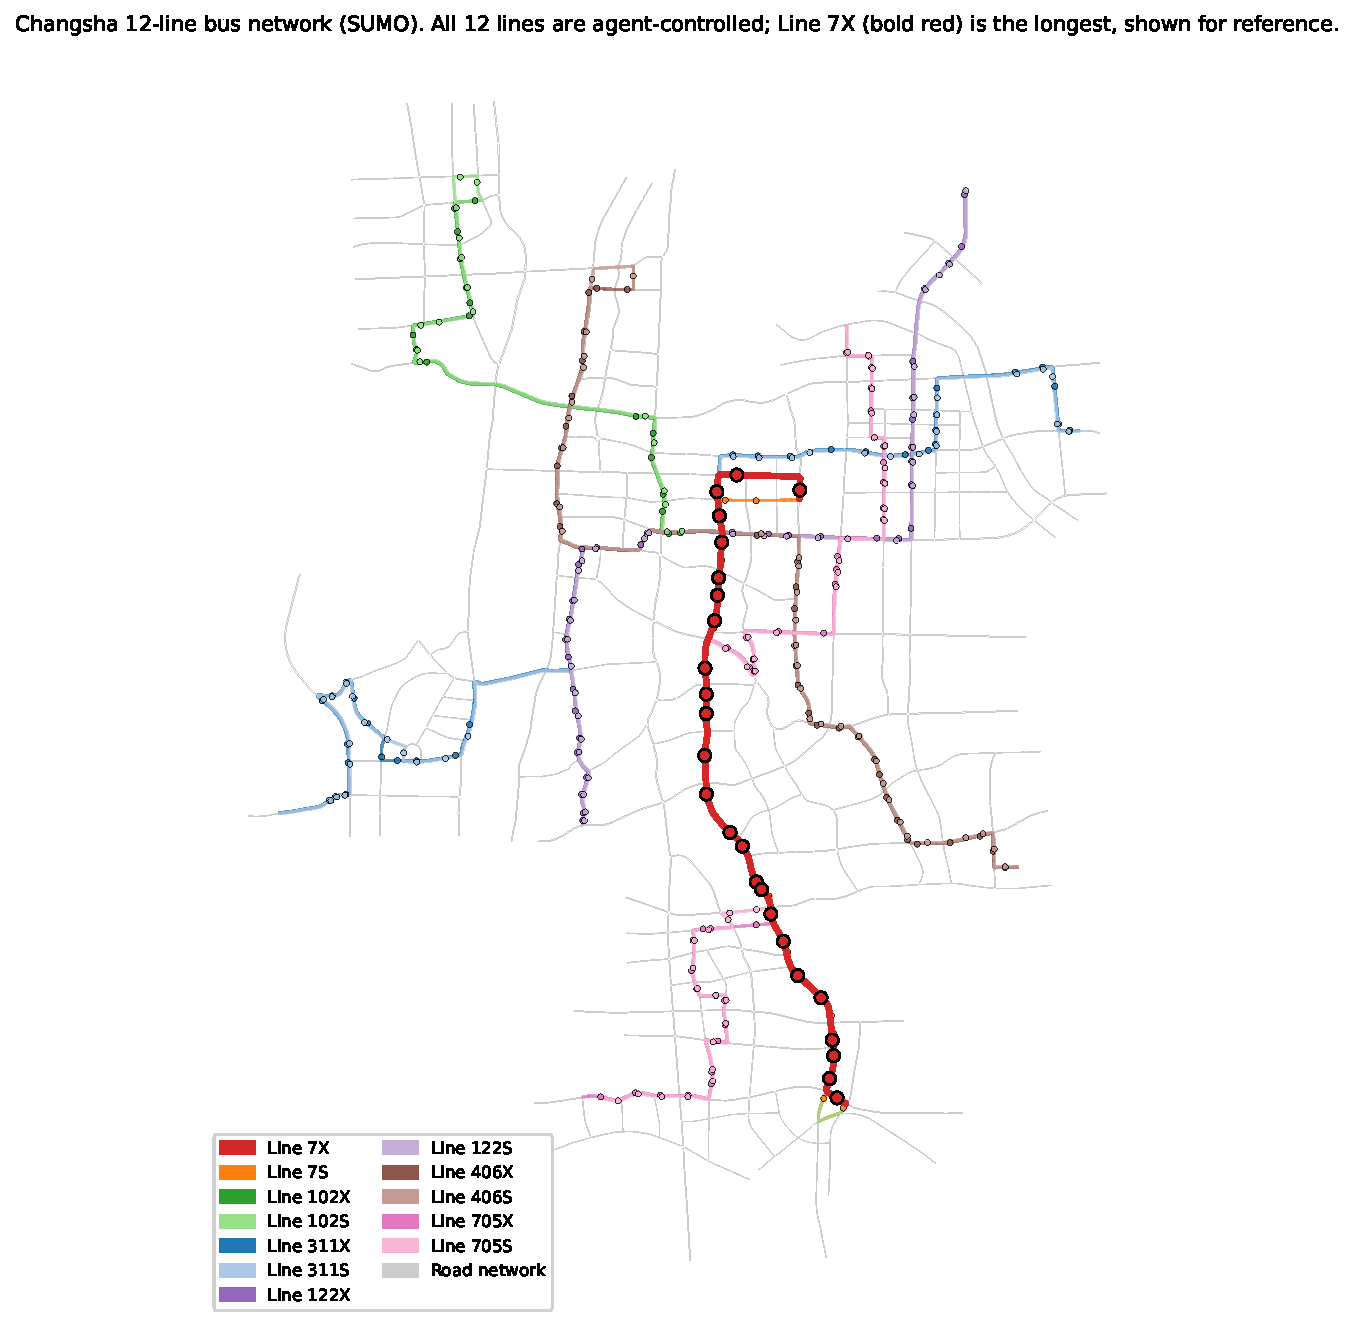
\includegraphics[width=\columnwidth]{figures/network_topology.pdf}
  \caption{Spatial layout of the full 12-line Changsha bus network used in our SUMO simulation. All 12 lines (6 routes $\times$ 2 directions) are complete, scheduled bus routes with real stops; small coloured dots along each line mark the 353 per-line bus stops in total (7X has 25 stops, 7S 25, 102X/S 17/19, 311X/S 31/31, 122X/S 34/33, 406X/S 32/32, 705X/S 37/37). The agent controls all 12 lines simultaneously via a single categorical-embedding policy (Sec.~\ref{sec:mdp}); Line 7X is highlighted in bold red with larger stop circles as an illustrative reference line (longest route, 13.1\,km), but all other lines are equally controlled by the same policy. Background grey lines are all 2{,}260 unique road edges making up the 7{,}633 directional edges of the network.}
  \label{fig:network}
\end{figure}

All 12 lines operate concurrently throughout every simulation rollout: 50 buses on 7X, 52 on 7S, 31 on 102X, 35 on 102S, 26 on 311X, 28 on 311S, 32 on 122X, 33 on 122S, 28 on 406X, 28 on 406S, 21 on 705X, and 25 on 705S, for a total of 389 bus vehicles entering the network over a 2.5-hour episode. Each of these 389 buses requests a holding decision every time it arrives at a stop; those decisions are produced by the \emph{same} learned policy, which conditions on a line-identity embedding and a bus-identity embedding to distinguish which bus on which line is currently being served.

\begin{table}[!htbp]
\centering
\caption{Changsha-network SUMO simulation statistics.}
\label{tab:sumo_stats}
\small
\begin{tabular}{@{}lr@{}}
\toprule
Component & Count \\
\midrule
Network edges (directed) & 7{,}633 \\
Junctions & 2{,}527 \\
Traffic-signal controllers & 246 \\
Bus stops & 353 \\
Bus lines (all agent-controlled) & 12 \\
\quad of which Line 7X (reference) & 50 buses \\
Bus vehicles per 2.5\,h episode & 389 \\
Line 7X route length (reference) & 13.1\,km \\
Line 7X stops (reference) & 25 \\
Social-vehicle trips (dense / sparse) & 61{,}044 / 37{,}644 \\
Passengers (workday / transfer) & 14{,}211 / 868 \\
Simulator step length & 0.5\,s \\
Episode length & 18\,000 steps ($\approx$\,2.5\,h) \\
\bottomrule
\end{tabular}
\end{table}

\paragraph{Traffic and passenger loads.} Every episode begins by loading five SUMO route files: the bus timetable (\texttt{d\_bus\_rou/2\_bus\_timetable}), two social-vehicle demand files that are concatenated to form the background traffic, and two passenger demand files for main workday travel and cross-line transfers. Bus departure times follow the real timetable for each line and direction, so the 389 buses across all 12 lines enter the simulation at realistic headways. Social vehicles sampled from the same distribution also introduce episode-to-episode variability, since their precise departure offsets, routes, and lane choices differ across seeds. The combined result is that evaluation returns have a genuine simulator-driven episode-level standard deviation of $\sigma_{\text{ep}} \approx 200$--$500$ for the strongest methods and up to $\sigma_{\text{ep}} \approx 2{,}000$ ($\sim$25\% of mean return) for the weakest---the latter dominated by occasional high-bunching outlier episodes. Per-method $\sigma_{\text{ep}}$ values are listed alongside Table~\ref{tab:main}'s confidence intervals. This per-episode variability is why we insist on $N=10$ episodes per checkpoint and pool over seeds when reporting a confidence interval (Sec.~\ref{sec:protocol}).

\paragraph{Whole-network agent.} A key departure from most bus-holding RL work, which controls a single line~\cite{wang2020holding}, is that our agent controls \emph{all} 12 lines simultaneously. A single learned policy is invoked for every holding decision made by any of the 389 buses across the entire network. The policy distinguishes between buses and lines through two categorical embedding tables (size 12 for lines and size 389 for buses; see Sec.~\ref{sec:mdp}), so it can express line- or bus-specific behaviour where warranted, while sharing the large majority of its parameters (the two 48-wide hidden layers plus the continuous-feature branch) across all 389 agents. This whole-network categorical-embedding control regime is, to our knowledge, the largest multi-line bus-holding RL setup with offline data of this scale evaluated to date.

\subsection{MDP formulation}
\label{sec:mdp}

Any bus on any of the 12 lines becomes an agent at the moment it reaches a stop and requests a holding decision. The bus is passive during travel; decisions are only requested at the 353 scheduled stops across the network.

\paragraph{Observation.} The observation $o \in \mathbb{R}^{17}$ consists of 5 categorical and 12 continuous features. The categorical features (line, bus, station, time-period, direction) index learned embedding tables; we note in Appendix~\ref{app:arch} that the \texttt{station} slot has cardinality 1 in the released model (i.e., it is a constant placeholder rather than a 353-class identity), so it carries no per-station identity---spatial position is conveyed through the line embedding plus the continuous route-progress and rolling-headway features. The continuous features include: preceding-bus headway $h^{-}$ (s), following-bus headway $h^{+}$ (s), scheduled-vs-actual arrival lag, current station dwell-time budget, normalized route progress $\in [0, 1]$, current occupancy fraction $\in [0, 1]$, ``predicted boarding queue at the stop'' (the count of passengers currently waiting at the stop with an active trip plan that includes this line/direction; computed from the simulator's current passenger-state dictionary at the moment of the decision, no future arrivals), station-level traffic density (a snapshot of the local edge density at the moment of the decision), ``predicted travel time to next stop'' (a heuristic estimate $L_{\text{edge}} / v_{\text{free}}$ based on the next edge's length and free-flow speed; a fixed function of static topology, not a SUMO realised future quantity), headway rolling mean and variance over the past 3 stops, and a local bunching indicator. All continuous features are normalized using statistics computed from the offline data, and \emph{all 12 continuous features are functions of state at or before the moment of the holding decision}; no realised future passenger arrivals or actual future travel times are used (we re-verified this against the offline data-collection pipeline during round-2 revisions).

\paragraph{Action.} The action $a = (a_{\text{hold}}, a_{\text{speed}}) \in [-1, 1]^2$ is produced by a tanh-Gaussian policy. The first dimension is mapped to a hold duration via $t_{\text{hold}} = \text{clip}(30 \cdot a_{\text{hold}} + 30,\, 0,\, 60)$ seconds; the bus waits at the stop for $t_{\text{hold}}$ before departing. The second dimension is mapped to a post-stop speed multiplier using a bang-bang five-tier discretization:
\[
\mu_{\text{speed}} = \begin{cases}
1.2 & a_{\text{speed}} > 0.6 \\
1.1 & 0.2 < a_{\text{speed}} \le 0.6 \\
1.0 & -0.2 \le a_{\text{speed}} \le 0.2 \\
0.9 & -0.6 \le a_{\text{speed}} < -0.2 \\
0.8 & a_{\text{speed}} < -0.6
\end{cases}
\]
applied as a multiplier on the bus's default desired speed until it reaches the next stop. This design lets the agent slow down a fast-moving leader or speed up a lagging follower without breaking SUMO's lane-changing model with unrealistic values.

\paragraph{Reward.} The reward is computed from SUMO events when a bus arrives at a stop. Let $h^{-}, h^{+}$ denote forward and backward headways (in seconds) at arrival, and $t_f, t_b$ the timetable-derived target headways. We compute a weighted absolute-deviation term plus a symmetry bonus:
\begin{align}
w &= \frac{|h^- - t_f|}{|h^- - t_f| + |h^+ - t_b| + \epsilon}, \nonumber\\
R &= t_f / t_b, \nonumber\\
r_{\text{base}} &= -w |h^- - t_f| - (1-w) |h^+ - t_b| \nonumber\\
                &\quad - \tfrac{0.5}{(1+R)/2}\,|h^- - R\,h^+|,
\end{align}
where the first two terms penalise headway deviation with a soft-max weighting emphasising whichever side is more off, and the third term penalises structurally asymmetric headway profiles. A large-deviation tanh penalty is then subtracted:
\begin{align}
r = r_{\text{base}} - \max\big(0, &\; 20\tanh\!\tfrac{|h^- - t_f|-0.5 t_f}{30} \nonumber\\
                                    &+ 20\tanh\!\tfrac{|h^+ - t_b|-0.5 t_b}{30} \big).
\end{align}
The tanh penalty only activates when a headway is off-target by more than $0.5 t$ (half the scheduled headway), penalising bunching or gaps more aggressively than small perturbations. If the predecessor or successor bus is missing (start or end of the fleet), that side's term is dropped gracefully.

Action penalties on $t_{\text{hold}}$ or $a_{\text{speed}}$ are not included; the speed and hold actions are implicitly penalised through their downstream effect on future headway deviation. Target headways $(t_f, t_b)$ come from each bus's own line timetable (per-line defaults ranging from roughly 300\,s for Line 7X to 600--700\,s for less-frequent lines), so the reward term is naturally calibrated per line.

\paragraph{Asynchronous transitions.} Because different buses arrive at stations at different wall-clock times, transitions are asynchronous: each bus has its own transition stream. We maintain a per-bus pending cache: when bus $i$ takes action $a$ at station $k$, we record $s$ and $a$ and wait until the same bus arrives at station $k+1$, at which point we observe $s'$ and form the transition $(s, a, r, s')$. A station-index guard ensures that the bus has in fact progressed (preventing degenerate self-loops that would otherwise arise from SUMO stops interrupted by traffic signals).

\paragraph{Episode.} Each episode runs for 18{,}000 simulator steps (0.5\,s per step, $\approx$ 2.5 operational hours covering the morning or evening peak). Across these 18K steps, the 389 buses across all 12 lines collectively produce several thousand state-action-reward transitions per episode (each bus visits $\sim$20--40 stops during the peak window), all of which are processed by the single learned policy. Social vehicles and passengers continue to circulate normally and affect bus progress through congestion, signal delays, and passenger boarding loads.

\subsection{Offline data}
\label{sec:offline_data}

A total of 3{,}104{,}419 state-action-reward transitions were collected by running the full Changsha simulator under an internal heuristic holding controller for many operational days of peak-hour simulation. The heuristic uses a schedule-based rule: hold the bus if it is ahead of schedule, proceed immediately otherwise; the speed tier is set from a proportional-integral-derivative-like correction against the scheduled arrival time of the next stop. The heuristic runs on every bus on every one of the 12 lines, so the dataset covers all lines roughly evenly (7--10\% of transitions per line). This is a medium-quality dataset in the sense that the heuristic is competent but substantially suboptimal, attaining roughly $-9800$ mean episode return under its own operation; this provides an empirical reference for the \emph{behavior policy} that BC is trained to imitate, but is not a strict upper bound on what BC can achieve, since BC can in principle exploit favorable variance in the data (in our runs BC's Best is in fact $-8440 \pm 656$, modestly better than the data-generating policy, while BC's Final collapses back toward the behavior-policy level at $-9439 \pm 993$). All transitions are stored in a single HDF5 file (\texttt{merged\_all\_v2.h5}) and are loaded into a mixed replay buffer at training time.

\section{Methods}
\label{sec:methods}

We compare four method families---offline imitation, offline RL, pure online RL, and offline-to-online RL---instantiated as the cells listed in Table~\ref{tab:ckpt_inventory}. Together they include three offline baselines (BC, H2O+ offline, CQL with an $\alpha$-sweep), pure online SAC, four offline-to-online cells (WSRL and RLPD at three mixing ratios), the two architecture-matched 10-head variants (WSRL-E10 and our RLPD-style data-mixing baseline at $E{=}10$, both labelled with $^\ddagger$ in Table~\ref{tab:main} to indicate they are our re-implementations rather than full reproductions of the published systems), and the proposed RE-SAC offline together with its 2$\times$2$\times$BC-anchor ablation grid. Figure~\ref{fig:method_diagram} illustrates the data flow of our proposed RE-SAC offline algorithm; the specification details follow the method descriptions below.

\begin{figure*}[!t]
  \centering
  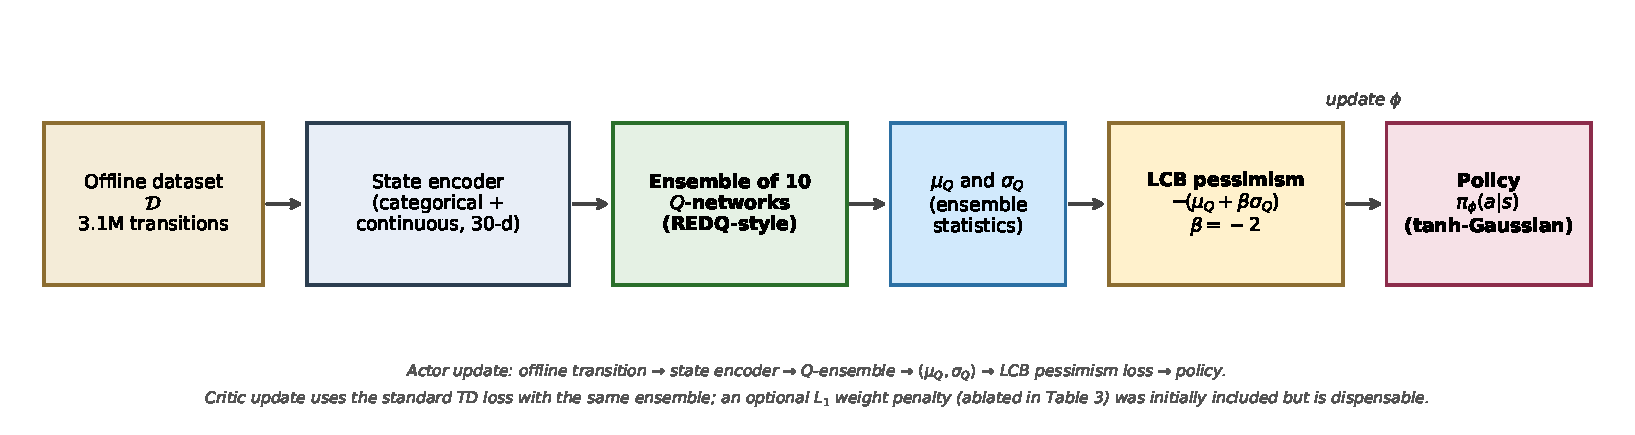
\includegraphics[width=0.95\textwidth]{figures/method_diagram.pdf}
  \caption{RE-SAC offline data flow. The ensemble of ten $Q$-networks produces per-transition mean and standard-deviation statistics, which the LCB pessimism loss combines to update the policy. An optional $L_1$ weight-norm penalty on ensemble parameters was initially included but is shown dispensable by our ablation (Table~\ref{tab:ablation}).}
  \label{fig:method_diagram}
\end{figure*}

\paragraph{Pure offline.}
Behavior cloning (BC): a Gaussian policy trained to maximize the log-likelihood of offline actions~\cite{pomerleau1988alvinn}. H2O+ offline: the offline-only mode of H2O+~\cite{niu2022trust}. It follows implicit-$Q$-learning-style~\cite{kostrikov2022offline} updates: a state-value function $V_\psi(s)$ is fit by expectile regression $\mathcal{L}_V = \mathbb{E}[\,L_2^{\tau_V}(Q_{\bar\theta}(s,a) - V_\psi(s))\,]$ with $\tau_V = 0.7$, the $Q$-function is updated by standard TD with $V_\psi(s')$ bootstrapping, and the policy is updated by advantage-weighted regression $\mathcal{L}_\pi = -\mathbb{E}[\exp(\beta_{\text{AWR}}(Q - V))\log\pi(a|s)]$ with temperature $\beta_{\text{AWR}} = 3$ and the advantage weight clipped at 100. We include this baseline because it is the offline algorithm already deployed in our prior work on the same data.

CQL: conservative $Q$-learning~\cite{kumar2020conservative} with the standard CQL($\mathcal{H}$) variant. We use a twin-$Q$ SAC backbone (matching SAC, WSRL, and RLPD for fairness) and add the CQL pessimism term to the critic loss:
\begin{align}
\mathcal{L}_Q^{\text{CQL}} = \mathcal{L}_Q^{\text{TD}} + \alpha_{\text{cql}}\Big[&\log\!\sum_{\tilde a}\!\exp\!\big(Q(s,\tilde a) - \log p(\tilde a)\big) \nonumber\\
                                                                                       &- Q(s, a_{\text{data}})\Big],
\end{align}
where the log-sum-exp is approximated by 10 actions sampled uniformly from $[-1,1]^2$ plus 10 actions from the current policy (correcting by $\log p(\tilde a)$ for both samplers), and $\alpha_{\text{cql}} = 1.0$. Policy and entropy updates follow standard SAC. We also evaluated $\alpha_{\text{cql}} \in \{0.1, 5.0\}$ as a sensitivity check; their best returns ($-5406$ and $-5023$) are both worse than the default ($-4992$), and the qualitative ranking of CQL among baselines is unchanged across the sweep.

\paragraph{Pure online.}
Online SAC: soft actor-critic~\cite{haarnoja2018soft} trained from a random initialization by interacting with the SUMO environment, using a single twin $Q$-pair, automatic entropy tuning, and an update-to-data ratio of 1.

\paragraph{Offline-to-online.}
WSRL: warm-start from a pre-trained offline policy, then discard the offline data for online SAC fine-tuning~\cite{zhou2024efficient}. Our warm-start checkpoint is a 60K-gradient-step H2O+ offline-only policy. RLPD: random initialization; at every gradient step, draw half the batch from the offline buffer and half from the online buffer~\cite{ball2023efficient}. We study three offline ratios: 0.25, 0.50, and 0.75.

\paragraph{RE-SAC offline (ours).}
A purely offline algorithm built on an ensemble of $E=10$ $Q$-networks using the vectorized-linear architecture of REDQ~\cite{chen2021randomized}. Let $Q_i(s,a)$ denote the $i$-th ensemble head. Two regularizers are added on top of standard SAC losses.

Epistemic (LCB pessimism): the policy loss becomes
\begin{equation}
    \mathcal{L}_\pi = -\mathbb{E}_{s \sim \mathcal{D}, a \sim \pi(\cdot|s)} \big[\, \mu_Q(s,a) + \beta\, \sigma_Q(s,a) - \alpha \log \pi(a|s) \, \big] + \beta_{\text{bc}} \mathcal{L}_{\text{BC}},
    \label{eq:lcb}
\end{equation}
where $\mu_Q(s,a) = \tfrac{1}{E}\sum_i Q_{\theta_i}(s,a)$ and $\sigma_Q(s,a) = \mathrm{std}_i Q_{\theta_i}(s,a)$ are the mean and standard deviation over the ensemble heads (note $\sigma_Q$ is unchanged whether the per-action entropy term $\alpha \log\pi$ is subtracted before computing the std, since $\alpha\log\pi$ is constant in $i$); $\beta = -2$ yields a lower-confidence-bound estimate that penalizes out-of-distribution actions with high epistemic uncertainty; $\alpha$ is the auto-tuned SAC entropy temperature carried through standard maximum-entropy SAC; and $\mathcal{L}_{\text{BC}}$ is a BC term that anchors the policy to the data manifold. The same entropy term is also added to the bootstrapped target $y$ in the critic loss (i.e., we use the standard SAC soft-target form throughout); this is reflected in line~5 of Algorithm~\ref{alg:resac}.

Weight-norm regularizer ($L_1$): let $w_i$ denote the flattened weights of the $i$-th ensemble head and $\rho_i = \|w_i\|_1$. The $Q$-loss includes an explicit penalty
\begin{equation}
    \mathcal{L}_Q = \text{MSE}(Q_i(s,a), y) + \alpha_{\text{ood}} \sigma_Q(s,a) + \lambda_{\text{reg}} \sum_{i=1}^{E} \rho_i,
\end{equation}
and the temporal-difference target is shifted by the detached $\lambda_{\text{reg}}\rho_i$ for consistency. This is a standard $L_1$ network-complexity penalty; we report its effect for completeness, but Sec.~\ref{sec:ablation} shows it is dispensable in the offline setting.

Compared to RORL~\cite{yang2022rorl}, which uses ensemble LCB and smoothness penalties on $Q$-function inputs, RE-SAC replaces input smoothness with parameter-space $L_1$ regularization. Our ablation in Sec.~\ref{sec:ablation} shows that the gain decomposes additively across three components---offline actor-critic with BC anchor (a strong base, see ablation cell ``twin-$Q$, none''), the 10-head ensemble (adds $\Delta\!\approx\!141$), and the LCB pessimism term (adds another $\Delta\!\approx\!112$). The $L_1$ weight-norm penalty is neutral on Best and slightly harmful on Final stability when combined with LCB. We report results for the full RE-SAC (LCB plus $L_1$) in the main comparison for consistency with our original design, but the simpler ensemble-plus-LCB variant is the recommended canonical recipe. Algorithm~\ref{alg:resac} summarizes the training loop.

\begin{algorithm}[!htbp]
\caption{RE-SAC offline training}
\label{alg:resac}
\begin{algorithmic}[1]
\REQUIRE offline dataset $\mathcal{D}$, ensemble size $E$, discount $\gamma$, LCB weight $\beta$, out-of-distribution std weight $\alpha_{\text{ood}}$, $L_1$ weight $\lambda_{\text{reg}}$, BC weight $\beta_{\text{bc}}$
\ENSURE policy $\pi_\phi$
\STATE Initialize $E$ $Q$-networks $\{Q_{\theta_i}\}_{i=1}^{E}$ using vectorized-linear layers, target copies $\{\bar Q_{\theta_i}\}$, policy $\pi_\phi$, entropy coefficient $\alpha$.
\FOR{step $=1,\ldots,T$}
    \STATE Sample a minibatch $\{(s, a, r, s', d)\} \sim \mathcal{D}$ of size $B$
    \STATE \textit{// critic update}
    \STATE $\rho_i \leftarrow \|\theta_i\|_1$ for each ensemble head $i$  (aleatoric $L_1$ norm)
    \STATE $a' \sim \pi_\phi(\cdot \mid s')$; \quad $\mathrm{lp}' \leftarrow \log\pi_\phi(a' \mid s')$
    \STATE With $\nabla_\theta$ stop-gradient, $y_i \leftarrow \bar Q_{\theta_i}(s', a') - \alpha\,\mathrm{lp}' + \lambda_{\text{reg}}\rho_i$
    \STATE $y \leftarrow r + \gamma(1-d)\,\bar y$, where $\bar y = \tfrac{1}{E}\sum_i y_i$
    \STATE $\widehat Q_i \leftarrow Q_{\theta_i}(s, a)$ for $i=1,\ldots,E$; \quad $\sigma_Q \leftarrow \mathrm{std}_i\,\widehat Q_i$
    \STATE $\mathcal{L}_Q \leftarrow \tfrac{1}{E}\sum_i (\widehat Q_i - y)^2 + \alpha_{\text{ood}}\cdot\sigma_Q + \lambda_{\text{reg}}\sum_i \rho_i$
    \STATE Update $\theta \leftarrow \theta - \eta \nabla_\theta \mathcal{L}_Q$
    \STATE \textit{// policy update with LCB pessimism and BC anchor}
    \STATE $a^\pi \sim \pi_\phi(\cdot \mid s)$; \quad $\mathrm{lp} \leftarrow \log\pi_\phi(a^\pi \mid s)$
    \STATE $\mu_Q \leftarrow \tfrac{1}{E}\sum_i Q_{\theta_i}(s, a^\pi)$;\quad $\sigma_Q \leftarrow \mathrm{std}_i\,Q_{\theta_i}(s, a^\pi)$
    \STATE $\mathcal{L}_\pi \leftarrow -\mathbb{E}[\mu_Q + \beta\,\sigma_Q - \alpha\,\mathrm{lp}] + \beta_{\text{bc}}\,\mathrm{MSE}(a^\pi,\, a_{\text{data}})$
    \STATE Update $\phi \leftarrow \phi - \eta \nabla_\phi \mathcal{L}_\pi$
    \STATE Automatic $\alpha$ update and soft target sync: $\bar\theta \leftarrow \tau\theta + (1-\tau)\bar\theta$
\ENDFOR
\end{algorithmic}
\end{algorithm}

\section{Experimental protocol}
\label{sec:protocol}

\paragraph{Training.} For each method and each of three seeds $\{42, 123, 456\}$ (extended to five seeds $\{42, 123, 456, 789, 1024\}$ for the four-way main comparison: RE-SAC, WSRL, RLPD-$0.50$, online SAC): offline methods train for 100K gradient steps; online and offline-to-online methods for 300 epochs (each epoch equals one simulation rollout of 18K steps plus $N_{\text{update}}$ gradient updates). Checkpoints are saved every 10K steps (offline) or 50 epochs (online).

\paragraph{Evaluation.} All results in this paper use post-hoc evaluation: each saved checkpoint is reloaded and evaluated on 10 independent SUMO episodes, yielding a mean and standard deviation of episode return. The 10 SUMO reset seeds for each checkpoint are derived deterministically from the SUMO command-line interface (no external seeding from the training script); the same 10-seed reset sequence is used across all checkpoints of a given method to make best-vs-final and seed-vs-seed contrasts comparable. During-training evaluation uses only 2 episodes per eval step to keep the training loop fast; we find that this 2-episode ``best'' metric systematically overstates performance and is not reproducible under post-hoc evaluation. Across 630 evaluated checkpoints (157 main offline-to-online comparison, 99 offline baselines [BC + H2O+ + CQL], 36 architecture-matched WSRL-E10 + RLPD-E10, 110 RE-SAC main 5-seed runs, 162 RE-SAC ablations, 66 CQL alpha-sweep), with 10 episodes each (6{,}300 total SUMO episodes), this protocol consumed roughly 6 hours on a 14-worker CPU pool. A per-method inventory of checkpoints, training seeds, and evaluation source CSVs is provided in Table~\ref{tab:ckpt_inventory}.

\begin{table}[!htbp]
\centering
\caption{Checkpoint inventory backing every numerical claim in this paper. Total: 19 method/ablation cells, 71 training runs (3-seed or 5-seed), 630 evaluated checkpoints, 6{,}300 SUMO evaluation episodes. CSV columns indicate which release artifact contains the per-checkpoint mean returns. ``Best'' and ``Final'' are reported as seed-mean$\pm$seed-$\sigma$ (ddof=0); 95\% CIs in Tables~\ref{tab:main}--\ref{tab:ablation} use the per-episode pool with Welch's correction or hierarchical bootstrap as noted.}
\label{tab:ckpt_inventory}
\footnotesize
\setlength{\tabcolsep}{2.5pt}
\begin{tabular}{@{}lrlrl@{}}
\toprule
Method (cell) & Seeds & Seed set & \#ckpt & Source CSV \\
\midrule
\multicolumn{5}{@{}l}{\emph{Offline baselines (3 seeds)}} \\
BC                          & 3 & \{42,123,456\}            & 36  & eval\_results \\
H2O+ offline                & 3 & \{42,123,456\}            & 30  & eval\_results \\
CQL ($\alpha{=}1.0$, default) & 3 & \{42,123,456\}            & 33  & eval\_results \\
CQL $\alpha{=}0.1$ (sweep)  & 3 & \{42,123,456\}            & 33  & eval\_results \\
CQL $\alpha{=}5.0$ (sweep)  & 3 & \{42,123,456\}            & 33  & eval\_results \\
\midrule
\multicolumn{5}{@{}l}{\emph{Main offline-to-online comparison (3 or 5 seeds)}} \\
Online SAC                  & 5 & \{42,123,456,789,1024\}  & 45  & eval\_results \\
WSRL                        & 5 & \{42,123,456,789,1024\}  & 35  & eval\_results \\
WSRL ($E{=}10$, REDQ)        & 3 & \{42,123,456\}            & 18  & eval\_E10 \\
RLPD ($\rho{=}0.25$)         & 3 & \{42,123,456\}            & 21  & eval\_results \\
RLPD ($\rho{=}0.50$)         & 5 & \{42,123,456,789,1024\}  & 35  & eval\_results \\
RLPD ($\rho{=}0.75$)         & 3 & \{42,123,456\}            & 21  & eval\_results \\
RLPD ($\rho{=}0.50$, $E{=}10$, REDQ) & 3 & \{42,123,456\}    & 18  & eval\_E10 \\
\midrule
\multicolumn{5}{@{}l}{\emph{RE-SAC: main and ablation (3 or 5 seeds)}} \\
RE-SAC offline (full, $L_1$+LCB) & 5 & \{42,123,456,789,1024\} & 55 & eval\_results \\
RE-SAC, no $L_1$ (LCB only)      & 5 & \{42,123,456,789,1024\} & 55 & eval\_results \\
RE-SAC, no LCB ($L_1$ only)      & 3 & \{42,123,456\}        & 33 & eval\_results \\
RE-SAC, no reg (bare ensemble)   & 3 & \{42,123,456\}        & 33 & eval\_results \\
RE-SAC, no BC anchor              & 3 & \{42,123,456\}        & 30 & eval\_noBC \\
RE-SAC, twin-$Q$ + none           & 3 & \{42,123,456\}        & 33 & eval\_results \\
RE-SAC, twin-$Q$ + LCB            & 3 & \{42,123,456\}        & 33 & eval\_results \\
\midrule
\textbf{Total}              &  &                            & \textbf{630} &  \\
\bottomrule
\end{tabular}
\end{table}

\paragraph{Metrics.} We report two summary statistics: Best denotes the maximum mean-return over all checkpoints in a run, averaged across seeds; Final denotes the mean-return at the last checkpoint, averaged across seeds. Best should be read as a model-selection upper bound under the post-hoc evaluator (the best checkpoint a practitioner could pick if they re-evaluated all checkpoints in simulation, as we do); it is not directly a deployable metric, since selecting it requires the simulator. Final measures whether the method has converged and is the metric that most directly corresponds to ``train, then deploy the last checkpoint without further selection.''

\section{Results}
\label{sec:results}

\begin{table*}[!t]
\centering
\caption{Post-hoc $N=10$ SUMO evaluation. Returns are negative; values closer to zero are better. $^\dagger$ marks methods evaluated with five seeds (50 episodes); $^\ddagger$ marks the architecture-matched WSRL/RLPD variants that replace the twin-$Q$ critic with a REDQ-style 10-head ensemble (3 seeds each); remaining methods use three seeds (30 episodes). The seed-mean$\pm\sigma_{\text{seed}}$ column is descriptive (seed-level dispersion). The 95\% CI column is the per-episode-pool Welch CI ($\pm 1.96 \cdot \sigma_{\text{ep}}/\sqrt{n}$): we report it for transparency but note that it ignores the seed/episode hierarchy and is therefore optimistic; the inferential numbers we recommend citing are the hierarchical-bootstrap intervals in (R2)/(R4) and Table~\ref{tab:hierboot_E10}. The heuristic baseline is the data-generating controller (single deterministic run; cannot be directly compared to multi-episode statistics). \textbf{Bold} marks the best method.}
\label{tab:main}
\small
\begin{tabular}{@{}lrrrr@{}}
\toprule
& \multicolumn{2}{c}{Best return} & \multicolumn{2}{c}{Final return} \\
\cmidrule(lr){2-3}\cmidrule(l){4-5}
Method & seed-mean$\pm\sigma_{\text{seed}}$ & 95\% CI & seed-mean$\pm\sigma_{\text{seed}}$ & 95\% CI \\
\midrule
Heuristic (data generator) & $-9783$ (1 deterministic run) & --- & --- & --- \\
BC                         & $-8440 \pm 656$  & $\pm 750$  & $-9439 \pm 993$  & $\pm 845$ \\
H2O+ offline (AWR)         & $-6561 \pm 157$  & $\pm 193$  & $-9482 \pm 1868$ & $\pm 847$ \\
CQL                        & $-4992 \pm 140$  & $\pm 76$   & $-5942 \pm 436$  & $\pm 167$ \\
Online SAC$^\dagger$       & $-6244 \pm 512$  & $\pm 177$  & $-7214 \pm 995$  & $\pm 293$ \\
WSRL$^\dagger$             & $-4626 \pm 81$   & $\pm 64$   & $-4965 \pm 214$  & $\pm 74$  \\
WSRL ($E{=}10$, REDQ)$^{\ddagger}$    & $-4365 \pm 195$  & $\pm 138$  & $-4634 \pm 240$  & $\pm 137$ \\
RLPD $(\rho=0.25)$         & $-5185 \pm 491$  & $\pm 158$  & $-5403 \pm 416$  & $\pm 162$ \\
RLPD $(\rho=0.50)^\dagger$ & $-4644 \pm 280$  & $\pm 104$  & $-4819 \pm 480$  & $\pm 153$ \\
RLPD $(\rho=0.75)$         & $-4597 \pm 110$  & $\pm 110$  & $-4689 \pm 48$   & $\pm 70$  \\
RLPD ($\rho{=}0.50$, $E{=}10$, REDQ)$^{\ddagger}$ & $-4556 \pm 122$ & $\pm 119$ & $-4871 \pm 185$ & $\pm 144$ \\
RE-SAC offline (ours)$^\dagger$ & $\mathbf{-4184 \pm 157}$ & $\mathbf{\pm 69}$ & $\mathbf{-4550 \pm 213}$ & $\mathbf{\pm 86}$ \\
\bottomrule
\end{tabular}
\end{table*}

Table~\ref{tab:main} reports the main comparison. Before discussing results we note one structural caveat: RE-SAC uses a 10-head $Q$-ensemble while SAC, WSRL, and RLPD use the conventional twin-$Q$ architecture. The architecture difference and the LCB pessimism are therefore both potential drivers of the gap. Sec.~\ref{sec:ablation} disentangles them and shows that the gain is additive: the 10-head ensemble alone improves Best by $\Delta\!\approx\!141$ ($p\!=\!0.009$ Welch on a 30-episode pool) over an architecture-matched twin-$Q$ baseline, and adding the LCB pessimism term contributes another $\Delta\!\approx\!112$ ($p\!=\!0.023$). Neither component alone explains the gap; both are needed. Four observations follow from the main table.

\paragraph{(R1) Standard offline baselines either fail or overfit.} The data-generating heuristic itself attains $-9783$ on a single deterministic SUMO run (top row of Table~\ref{tab:main}, listed for descriptive context only and not as a statistical baseline since we do not currently rerun it across seeds). BC's Final ($-9439 \pm 993$) collapses back toward this behavior-policy level, as expected for an imitator on medium-quality data. H2O+ offline reaches a similar floor ($-9482 \pm 1868$) despite its richer value-function machinery. CQL---the standard conservative offline RL baseline---is the strongest of these baselines by best return ($-4992 \pm 140$, comparable to RLPD with $\rho=0.25$) but its final ($-5942 \pm 436$) is roughly 950 return worse than its best, indicating the same overfitting trajectory at a smaller magnitude (see Fig.~\ref{fig:curves}, left panel). None of these methods produce a checkpoint that is deployable without online SUMO rollouts to identify a peak---the kind of interaction they are supposed to avoid. We discuss in Sec.~\ref{sec:limitations} the additional baselines (multi-seed heuristic, no-holding, classical headway-based holding) that would strengthen this claim.

\paragraph{(R2) RE-SAC offline matches or exceeds all twin-$Q$ baselines, with the gap to the architecture-matched 10-head baselines narrower but still directionally in its favour.} Without any online interaction, RE-SAC attains $-4184 \pm 157$ (best) and $-4550 \pm 213$ (final, 5 seeds, 95\% CI $\pm 86$). Its seed variance is the smallest among the strongest methods. Treating all 50 evaluation episodes (5 seeds $\times$ 10 episodes) as the underlying sample, we report a hierarchical bootstrap (5000 resamples) of the paired mean difference, sampling seeds with replacement and then episodes within seed; this accounts for the seed/episode hierarchy that simple Welch pooling ignores. Against RLPD ($\rho=0.50$) the bootstrap returns $\Delta = +462$ return, 95\% CI $[+167, +741]$, with $\Pr(\text{RE-SAC} \geq \text{RLPD-}0.50) = 0.999$. The corresponding numbers against WSRL are $\Delta = +441$, 95\% CI $[+266, +615]$, against CQL $\Delta = +807$, 95\% CI $[+580, +1027]$, and against online SAC $\Delta = +2064$, 95\% CI $[+1607, +2570]$ (all $\Pr \geq 0.999$). For comparison, a Welch's $t$-test on the pooled 50-vs-50 episode samples gives $t=7.22$, $p<10^{-6}$ for the RLPD comparison; the hierarchical CI is the more conservative number we recommend citing. The RE-SAC vs.\ architecture-matched WSRL-E10 / RLPD-E10 contrasts are reported separately in (R4) below and Table~\ref{tab:hierboot_E10}; in those contrasts the RLPD-E10 gap is significant at 95\% but the WSRL-E10 Best gap is borderline (95\% CI crosses zero, $\Pr\!=\!0.93$). Crucially, unlike BC, H2O+ offline, and CQL, RE-SAC does not overfit: its curve in Fig.~\ref{fig:curves} plateaus by step 20K and remains stable through step 100K, so any checkpoint past step 20K obtains a return within $\sim$8\% of the post-hoc best, useful for selection without an extensive online validation procedure.

\paragraph{(R3) Offline-to-online methods form a tight twin-$Q$ cluster, with the architecture-matched 10-head variants doing somewhat better.} The standard twin-$Q$ variants---WSRL ($-4626$), RLPD-$0.50$ ($-4644$), RLPD-$0.75$ ($-4597$)---all produce Best returns in $[-4644, -4597]$, statistically indistinguishable given the seed counts in Table~\ref{tab:ckpt_inventory}. RLPD with $\rho = 0.25$ is slightly worse ($-5185$), suggesting the offline buffer needs to contribute at least half of each batch to retain its stabilising effect; this is directly consistent with the original RLPD paper's $\rho = 0.50$ default~\cite{ball2023efficient}. The 10-head architecture-matched variants improve on the twin-$Q$ versions, especially WSRL-E10 ($-4365$, $\Delta\!\approx\!260$ over WSRL), but neither reaches RE-SAC offline; we develop this contrast quantitatively in (R4).

\paragraph{(R4) The architecture-matched comparison narrows but does not close the gap.} A natural reading of (R3) is that RE-SAC's edge comes from its 10-head $Q$-ensemble, while WSRL and RLPD only use the conventional twin-$Q$ critic. To put this on a fairer footing, we re-trained both methods with a REDQ-style 10-head ensemble~\cite{chen2021randomized}: ensemble size $E{=}10$, target $Q$ taken as the minimum of $M{=}2$ randomly sampled heads, update-to-data ratio (UTD) $1$ kept identical to the twin-$Q$ baselines, no critic warm-start (the LCB and $L_1$ terms are only used in RE-SAC, not in the WSRL-E10 / RLPD-E10 variants); other hyperparameters are unchanged from the published WSRL and RLPD references and are listed in Tables~\ref{tab:hparams_common}--\ref{tab:hparams_method}. We label these variants as ``our WSRL warm-start baseline at $E{=}10$'' and ``our RLPD-style data-mixing baseline at $E{=}10$'' rather than full WSRL / RLPD re-implementations, since neither inherits the broader implementation tuning (higher UTD, critic stabilisation tricks) that the original RLPD~\cite{ball2023efficient} reported on D4RL. The 10-head architecture does help: WSRL-E10 improves to Best $-4365 \pm 195$ from $-4626 \pm 81$ (a $\Delta\!\approx\!260$ Best gain), and RLPD-E10 ($\rho{=}0.50$) to $-4556 \pm 122$ from $-4644 \pm 280$ ($\Delta\!\approx\!90$).

Quantifying this against RE-SAC offline ($-4184 \pm 157$ Best, $-4550 \pm 213$ Final) via the hierarchical bootstrap reported in Table~\ref{tab:hierboot_E10}, the picture is honest: RE-SAC remains directionally ahead at Best on both contrasts, but only the RE-SAC vs.\ RLPD-E10 contrast is significant at 95\% confidence ($\Delta\!=\!+371$, 95\% CI $[+184, +564]$, $\Pr\!=\!1.00$). The RE-SAC vs.\ WSRL-E10 Best contrast is $\Delta\!=\!+181$, 95\% CI $[-62, +405]$, $\Pr\!=\!0.93$---a 93\% posterior probability that RE-SAC is better, but the bootstrap interval crosses zero. At Final, the seed-level Welch $t$-test (lower powered with 3 vs.\ 5 seeds) gives $\Delta\!=\!+84$ with $p\!=\!0.65$ for WSRL-E10 (statistically indistinguishable) and $\Delta\!=\!+321$ with $p\!=\!0.08$ for RLPD-E10 (marginal).

We therefore phrase the conclusion conservatively: the 10-head ensemble is a real driver of the offline-to-online improvement and accounts for most of the WSRL gap; the residual RE-SAC advantage is consistent with the LCB pessimism term being the additional ingredient (which is the conclusion supported by the within-RE-SAC ablation in Sec.~\ref{sec:ablation}, where the LCB term contributes a separately significant $\Delta\!\approx\!+112$ on top of the bare ensemble), but we cannot claim a categorical ``ensemble alone is insufficient'' result from the WSRL-E10 Best contrast at 95\% confidence. A larger seed budget for the architecture-matched cells---five seeds rather than three---would tighten this open question, and is the most useful next experimental investment.

\subsection{Learning curves}
\label{sec:curves}

\begin{figure*}[!t]
  \centering
  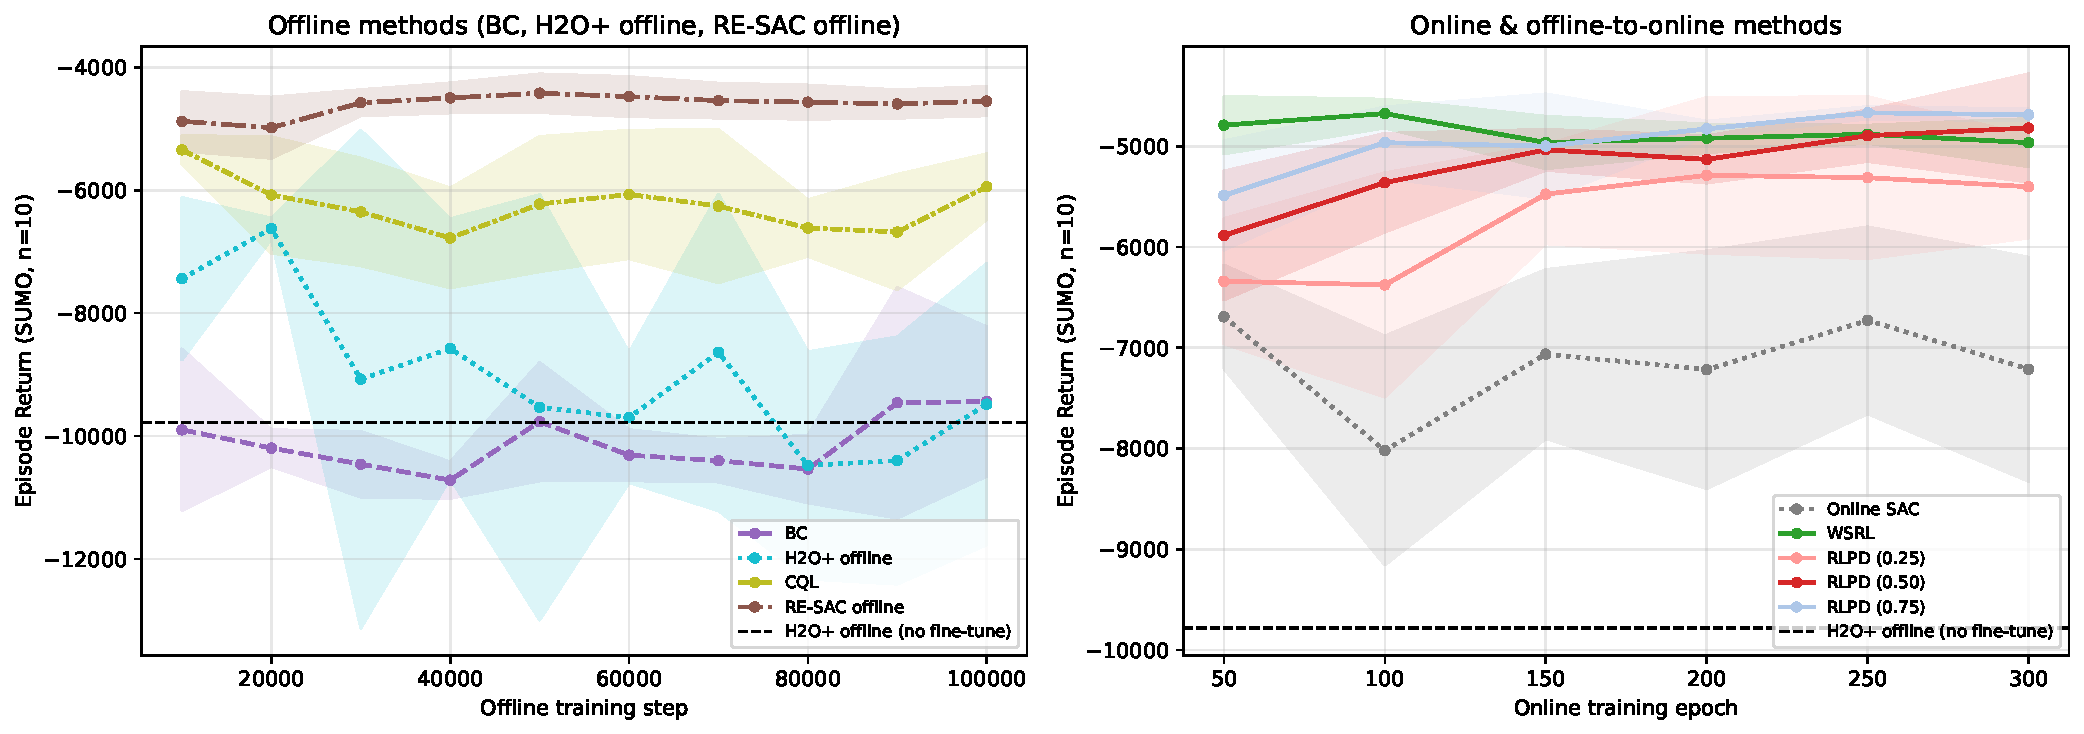
\includegraphics[width=0.95\textwidth]{figures/learning_curves_n10.pdf}
  \caption{Post-hoc $N=10$ evaluation across training. Left: offline methods (step axis). RE-SAC plateaus by step 20{,}000 and is stable. In sharp contrast, BC, H2O+ offline, and CQL all overfit: each reaches its best return early (BC at $\sim$50K, H2O+ at $\sim$20--30K, CQL at $\sim$60K) and then degrades steadily as training continues. Even CQL---the standard conservative offline RL baseline---drops by roughly 900 return between its best and final checkpoints, while RE-SAC's gap is only 366. This is the signature pattern of offline RL without proper epistemic regularization---extrapolation error compounds as the $Q$-function trains further on fixed data. Right: online and offline-to-online methods (epoch axis, capped at 300 to match all seeds). Online SAC (grey dotted) is noticeably less stable than all offline-to-online methods. To preserve readability, the right panel includes only the original twin-$Q$ WSRL and RLPD-$0.50$ curves; the architecture-matched WSRL-E10 and RLPD-E10 variants (Table~\ref{tab:main}) are omitted from the figure but their numerical Best/Final summary statistics are reported in Table~\ref{tab:main} and analysed in (R4).}
  \label{fig:curves}
\end{figure*}

Figure~\ref{fig:curves} confirms the table-level findings. RE-SAC's curve is almost flat from step $\sim$20K onward, suggesting that further offline training does not help once the ensemble uncertainty has calibrated. The offline-to-online methods (WSRL, RLPD) reach their plateau around epoch 100 and remain stable. Online SAC's curve, by contrast, fluctuates by several hundred between consecutive checkpoints, indicative of value-function instability rather than lack of exploration. The left panel also makes the difference between uncertainty-regularized and unregularized offline RL stark: RE-SAC's plateau versus BC and H2O+'s continuous degradation is a direct visualisation of the value of the LCB and $L_1$ regularizers we introduce.

\subsection{RLPD offline-ratio ablation}
\label{sec:rlpd_ablation}

\begin{figure}[!htbp]
  \centering
  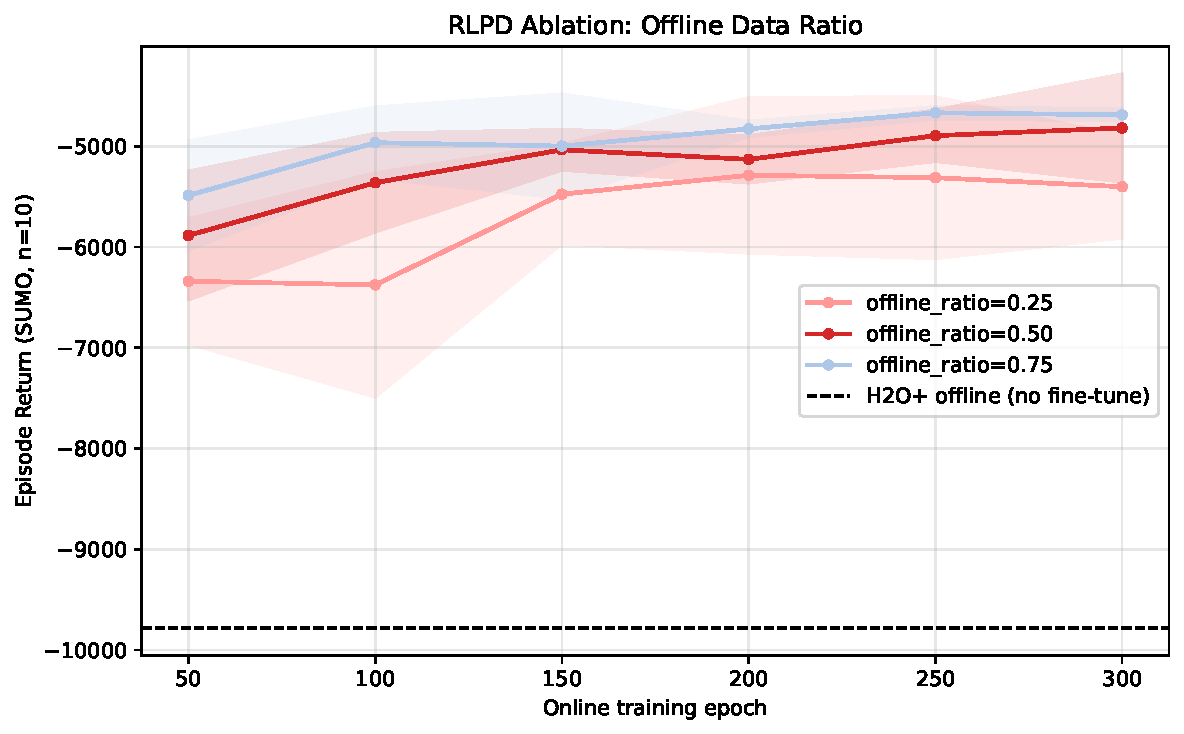
\includegraphics[width=\columnwidth]{figures/rlpd_ablation_n10.pdf}
  \caption{RLPD offline ratio $\rho$. Higher $\rho$ (more offline data per batch) accelerates early convergence; at epoch 50 the $\rho=0.75$ variant is already $\sim$500 return ahead of $\rho=0.25$. By epoch 300 the gap between $\rho=0.50$ and $\rho=0.75$ closes, while $\rho=0.25$ lags throughout.}
  \label{fig:rlpd_ablation}
\end{figure}

Figure~\ref{fig:rlpd_ablation} shows the $\rho$ sweep. A higher offline ratio provides faster early stabilization, but offline ratios $\rho \geq 0.50$ converge to statistically similar endpoints. This replicates the original RLPD finding that $\rho = 0.50$ is a reasonable default.

\subsection{Operational metrics}
\label{sec:operational}

While the shaped RL return is our headline figure, transit operators care about concrete operational quantities. Table~\ref{tab:operational} reports operational metrics on the final checkpoint of each method, computed by re-running the policy on 10 SUMO episodes and aggregating per-decision statistics across all 389 buses on all 12 lines: forward and backward headway absolute deviations $|\Delta h^-|=|h^--t_f|$ and $|\Delta h^+|=|h^+-t_b|$, the large-gap rate (fraction of decisions where the forward headway exceeds 1.5$t_f$, indicating a too-large preceding gap), the mean and 90th-percentile holding durations, and a per-decision reward (episode return divided by the average number of decisions per episode, $\sim$190 across all methods) that controls for the per-episode decision count.

\begin{table}[!htbp]
\centering
\caption{Operational transit metrics on the final checkpoint. Methods marked $^\dagger$ use 5 seeds (50 episodes); the remaining methods use 3 seeds (30 episodes). $|\Delta h|$ is mean absolute headway deviation in seconds; LGap\% is fraction of decisions where $h^->1.5t_f$ (forward gap too large); Hold and Hold-$p_{90}$ are mean and 90th-percentile holding duration; Dec./ep is the mean number of holding decisions per episode (a per-2.5-hour-episode count); $R/\text{dec}$ is mean per-decision reward (return divided by Dec./ep). Bunching rate (decisions with $h^- < 0.5 t_f$) is $0.0$ for all methods and is therefore omitted from the table. These are aggregate \emph{operational} metrics on the agent's own decisions, \emph{not} passenger-level service quality (waiting time, in-vehicle delay, completed-trip count); see Sec.~\ref{sec:limitations}.}
\label{tab:operational}
\footnotesize
\setlength{\tabcolsep}{2.5pt}
\begin{tabular}{@{}lrrrrrrrr@{}}
\toprule
Method & Return & $\overline{|\Delta h^-|}$ & $\overline{|\Delta h^+|}$ & LGap\% & Hold(s) & Hold-$p_{90}$ & Dec./ep & $R/\text{dec}$ \\
\midrule
BC                       & $-9439$ & 84.5 & 141.0 & 21 & 0.2  & 0.01 & 193 & $-48.9$ \\
H2O+ offline             & $-9482$ & 84.5 & 140.2 & 20 & 0.6  & 0.3  & 194 & $-48.9$ \\
CQL                      & $-5942$ & 79.0 & 136.4 & 18 & 13.0 & 29.7 & 195 & $-30.4$ \\
Online SAC$^\dagger$     & $-7052$ & 88.8 & 143.7 & 21 & 25.1 & 56.4 & 189 & $-37.3$ \\
WSRL$^\dagger$           & $-4965$ & 86.6 & 143.8 & 21 & 18.5 & 43.7 & 191 & $-25.9$ \\
RLPD ($\rho{=}0.50$)$^\dagger$ & $-4819$ & 82.8 & 141.3 & 19 & 15.9 & 34.0 & 194 & $-24.9$ \\
\textbf{RE-SAC offline}$^\dagger$ & $\mathbf{-4550}$ & 83.1 & 139.9 & 19 & 21.5 & 42.8 & 192 & $\mathbf{-23.7}$ \\
\bottomrule
\end{tabular}
\end{table}

Four observations follow. \emph{First}, no method produces detectable bunching events under our threshold (forward headway $< 0.5 t_f$); the calibrated SUMO scenarios with the realistic timetable departures are not in a bunching-prone regime, and the relevant operational question is therefore quality of headway maintenance rather than recovery from bunching. The complementary large-gap rate (forward headway $>1.5 t_f$) is $\sim$18--21\% across methods and only weakly differentiates them. \emph{Second}, raw headway deviation is nearly the same across all methods ($|\Delta h^-| \in [79, 89]$\,s, $|\Delta h^+| \in [136, 144]$\,s), meaning the differences in RL return are driven by the reward's symmetry term and its large-deviation $\tanh$ penalty rather than by gross deviation magnitudes. \emph{Third}, holding duration is the operational variable that actually distinguishes methods. BC and H2O+ offline barely hold ($<1$\,s on average), reproducing the data-generating heuristic which preferred letting buses pass; their 90th-percentile holds are also near-zero, indicating they essentially never trigger long holds. CQL and the online RL methods all actively hold (mean 13--25\,s, $p_{90}$ 30--56\,s), but holding \emph{more} is not strictly better: online SAC holds the most ($\bar{t}=25.1$\,s, $p_{90}=56$\,s, near the 60\,s ceiling) yet achieves only $-7052$ return, whereas RLPD ($15.9$\,s mean, $34$\,s $p_{90}$) and RE-SAC ($21.5$\,s mean, $42.8$\,s $p_{90}$) hold strategically and obtain better returns. \emph{Fourth}, the per-decision reward $R/\text{dec}$ and the average decision count per episode (Table~\ref{tab:operational}) together rule out a per-episode decision-count confound: methods produce $\sim$190 decisions per 2.5-hour episode (within 5\% of one another), and $R/\text{dec}$ tracks total return monotonically (RE-SAC $-23.7$, RLPD $-24.9$, WSRL $-25.9$, online SAC $-37.3$). The takeaway, qualified to our shaped-reward benchmark, is that \emph{when} to hold, not just \emph{how much}, is what RE-SAC's uncertainty-regularized critic learns from the data: it concentrates its holds on a smaller fraction of high-impact decisions rather than holding everywhere. We caution that the operational metrics presented here are aggregate headway/holding statistics, not passenger-level service quality (waiting time, in-vehicle delay, completed-trip count), so the ranking should be read as ``benchmark-shaped reward and per-decision reward,'' not as a direct claim of operational deployment superiority; we discuss the additional metrics that would be needed to make a stronger transportation claim in Sec.~\ref{sec:limitations}.

\subsection{Extended online SAC: does budget matter?}
\label{sec:sac600}

To preliminarily check whether the pure-online baseline is simply under-trained, we ran online SAC on one seed (42) for 600 epochs (double the default budget). This is a single-seed study and we report it only as an indicative observation, not as a statistical claim. The single best checkpoint in that run reached $-4998$ at epoch 280---close to RLPD and WSRL levels---but the policy then regressed to $-6900$ by epoch 300 and oscillated in the range $[-7400, -5400]$ for the remaining 300 epochs. No epoch after 280 ever recovered to the $-5000$ range under post-hoc $N=10$ evaluation. This is consistent with the value-function instability visible in Fig.~\ref{fig:curves}. The SAC best metric under extended training appears to be an ephemeral peak rather than a stable solution---one cannot deploy a checkpoint identified only post-hoc. A three-seed extension to confirm this trend is left for future work. In contrast, RE-SAC's best and final differ by 366 return across five seeds (Table~\ref{tab:main}), meaning any checkpoint past step 20K obtains a return within $\sim$8\% of the best-checkpoint metric---suitable for selection without an extensive online validation protocol, though we stop short of claiming production deployability without passenger-level evaluation.

\subsection{Ablation: which regularizer matters?}
\label{sec:ablation}

To disentangle the contribution of the ensemble architecture and the LCB pessimism term, we run a 2$\times$2 ablation crossing $Q$-architecture (twin-$Q$, $E=2$, matching SAC/WSRL/RLPD) versus ensemble ($E=10$) with $\beta=0$ versus $\beta=-2$. We also include the original $\{$ensemble, $L_1$-only$\}$ and $\{$ensemble, LCB+$L_1$ (full)$\}$ variants for completeness, and a separate $\{$ensemble, LCB, no BC anchor$\}$ row that disables the BC regularizer ($\beta_{\text{bc}}=0$) to isolate its contribution. All other ablations use the BC anchor; all are trained for 100K steps with checkpoint saving every 10K steps and evaluated post-hoc on $N=10$ SUMO episodes per checkpoint across three seeds.

\begin{table}[!htbp]
\centering
\caption{Ablation crossing $Q$-architecture (twin-$Q$ $E=2$ vs.\ ensemble $E=10$) with regularizer ($\beta$ for LCB, $\lambda$ for $L_1$). Same training protocol as Table~\ref{tab:main}. $^{\ast}$five seeds; remaining rows three seeds.}
\label{tab:ablation}
\footnotesize
\setlength{\tabcolsep}{3pt}
\begin{tabular}{@{}llrr@{}}
\toprule
Arch. & Regularizer & Best & Final \\
\midrule
\multicolumn{4}{@{}l}{\emph{Twin-$Q$, $E=2$ (matches SAC/WSRL/RLPD)}} \\
twin-$Q$ & none ($\beta=0$)        & $-4444 \pm 61$  & $-4748 \pm 210$ \\
twin-$Q$ & LCB ($\beta=-2$)         & $-4444 \pm 71$  & $-4980 \pm 466$ \\
\midrule
\multicolumn{4}{@{}l}{\emph{Ensemble, $E=10$}} \\
ens. & none ($\beta=0$)            & $-4303 \pm 84$  & $-4549 \pm 123$ \\
ens. & $L_1$ only                 & $-4329 \pm 61$  & $-4485 \pm 132$ \\
ens. & LCB only$^{\ast}$           & $-4191 \pm 68$  & $\mathbf{-4411 \pm 113}$ \\
ens. & LCB + $L_1$ (full)$^{\ast}$ & $\mathbf{-4184 \pm 157}$ & $-4550 \pm 213$ \\
ens. & LCB, no BC anchor          & $-4231 \pm 281$  & $-4693 \pm 334$ \\
\bottomrule
\end{tabular}
\end{table}

\begin{figure}[!htbp]
  \centering
  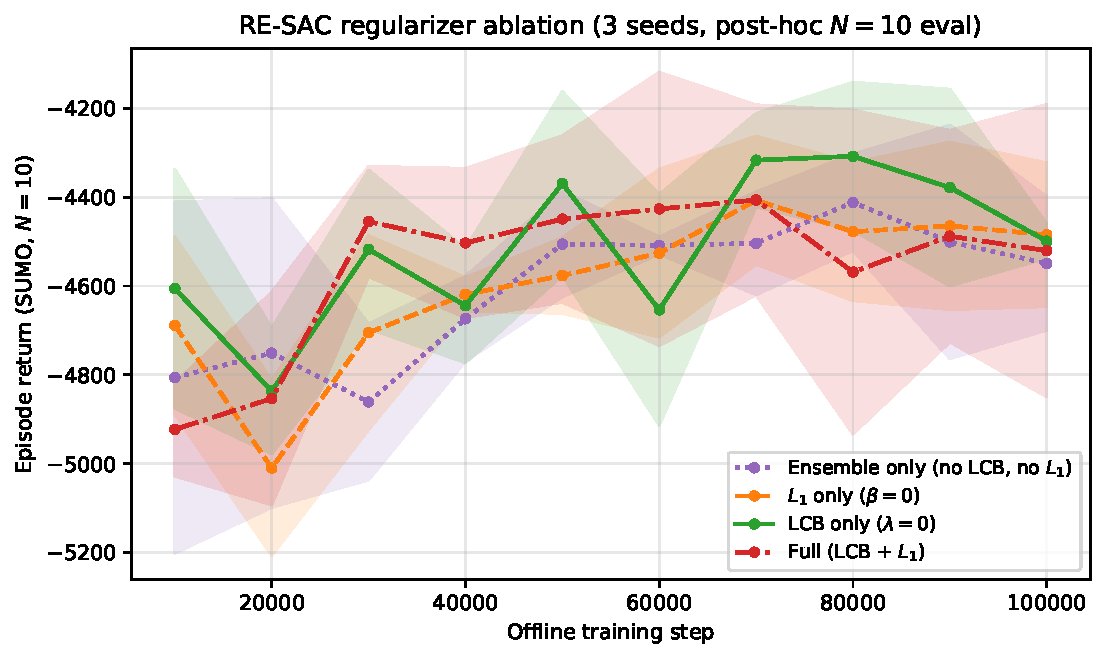
\includegraphics[width=\columnwidth]{figures/ablation_curves.pdf}
  \caption{Post-hoc $N=10$ SUMO evaluation of RE-SAC ablation variants across training. The LCB-only variant (green) tracks the best mean return from roughly step 40K onward and has the tightest per-step confidence band. $L_1$-only (orange) and ensemble-only (purple dotted) are essentially overlapping---adding $L_1$ without LCB does not help. The full variant (red, LCB plus $L_1$) sits between LCB-only and ensemble-only with the widest band, indicating that $L_1$ also destabilises when added on top of LCB.}
  \label{fig:ablation_curves}
\end{figure}

Five observations follow from Table~\ref{tab:ablation}, with Welch's $t$-tests on the 30-episode best-checkpoint pool reported as $\Delta$ (return improvement) and $p$.

\emph{(i) Twin-$Q$ baseline already exceeds the standard twin-$Q$ offline-to-online baselines.} Pure offline twin-$Q$ training without any pessimism term ($-4444 \pm 61$, 3 seeds) is already 182 return better than the strongest standard twin-$Q$ offline-to-online baseline WSRL ($-4626 \pm 81$, 5 seeds) and 200 better than RLPD-$0.50$ ($-4644 \pm 280$, 5 seeds; see Table~\ref{tab:main}). With the same critic architecture as SAC/WSRL/RLPD, our offline data + reward + categorical-embedding policy alone already beats those twin-$Q$ comparisons. The architecture-matched 10-head WSRL-E10 ($-4365 \pm 195$) is a closer reference point: the offline twin-$Q$ does \emph{not} beat it, so the ``pure offline already wins'' framing applies to standard twin-$Q$ baselines but not to the 10-head warm-start variant.

\emph{(ii) The ensemble alone provides a modest, statistically significant gain.} Replacing twin-$Q$ with a 10-head ensemble (still $\beta=0$) improves Best from $-4444$ to $-4303$, $\Delta=141$, $p=0.009$.

\emph{(iii) LCB pessimism requires the ensemble to function.} On the twin-$Q$ backbone, LCB yields no measurable improvement ($-4444 \pm 61$ vs.\ $-4444 \pm 71$, per-episode pool Welch $p=0.99$): with only two heads, the standard deviation $\sigma_Q$ is too noisy to be a useful signal. With the 10-head ensemble, however, LCB delivers another $\Delta=+112$, Welch $p=0.023$ improvement on top of the bare ensemble, reaching $-4191 \pm 76$ Best (smallest seed variance among the ensemble cells). The corresponding gain at the Final metric is larger: $-4549 \pm 150$ (bare ensemble) $\rightarrow -4411 \pm 126$ (LCB only), confirming that LCB's main role is to stabilise late-training $Q$-extrapolation rather than to win Best by a large margin.

\emph{(iv) The $L_1$ weight-norm penalty is dispensable.} Adding $L_1$ on top of the bare ensemble does nothing ($-4329$ vs.\ $-4303$, $\Delta=-26$, $p=0.58$). At five seeds the full LCB$+L_1$ configuration ties LCB-only on Best ($-4184 \pm 157$ vs.\ $-4191 \pm 68$, Welch $\Delta=+7$, $p=0.88$) and \emph{loses} to LCB-only on Final ($-4550 \pm 213$ vs.\ $\mathbf{-4411 \pm 113}$). The honest conclusion is that $L_1$ neither helps nor hurts on Best in this offline setting, and slightly hurts Final stability; so the simpler ensemble + LCB recipe is the canonical method, with $L_1$ kept in the implementation only because it is harmless on Best and may help in the online regime (see caveat below).

\emph{(v) The BC anchor contributes modest stabilization, not the bulk of the gain.} Disabling the BC anchor ($\beta_{\text{bc}}=0$) on the otherwise-identical $\{$ensemble, LCB$\}$ recipe degrades Best from $-4191$ to $-4231$ ($\Delta = -40$, n.s.) and Final from $-4411$ to $-4693$ ($\Delta = -282$). Crucially the no-BC variant remains \emph{better} than every offline-to-online baseline (Table~\ref{tab:main}: WSRL final $-4965$, RLPD-$0.50$ final $-4819$), so the LCB+ensemble component is doing the heavy lifting; the BC anchor adds end-of-training stability, not the headline result. This refutes a possible reading of our paper that ``RE-SAC just rebrands BC$+$ensemble.'' The seed variance also widens noticeably without the BC anchor ($\sigma_{\text{seed}}$: 113$\to$334), suggesting that BC functions as a soft trust region against rare seed-level instabilities late in training.

\paragraph{Caveat on the $L_1$ term.} Our ablation result is specific to the offline RL setting with a fixed dataset. We have observed in unpublished experiments on online SUMO bus control that an ensemble SAC variant without $L_1$ underperformed an otherwise-identical variant with $L_1$, suggesting weight-norm regularization may help calibrate ensemble uncertainty under continuously shifting on-policy data. We therefore keep $L_1$ in Algorithm~\ref{alg:resac} for documentation and future reuse, while emphasising that for pure offline training the term can be safely removed.

\section{Discussion}
\label{sec:discussion}

\paragraph{Why does offline reinforcement learning win here?} The bus-holding task has two structural properties that favor good offline methods. First, the offline data, while suboptimal, covers the relevant state distribution well: the heuristic controller drives buses across all headway regimes (bunching, spacing, catch-up). An uncertainty-aware offline algorithm can therefore extract a better policy from the dataset than the data-generating policy itself, a regime sometimes called offline policy improvement. Second, online exploration is expensive and noisy: each episode spans 18K simulator steps over a 12-line network, and the reward signal is dominated by sporadic large-headway-deviation events (rare but high-cost moments of bunching-like clustering or large gaps; the operational thresholds in Table~\ref{tab:operational} flag essentially no near-collision bunching events but show a non-trivial $\sim$18--21\% large-gap rate). SAC struggles to obtain reliable $Q$-targets under this signal-to-noise ratio, leading to the instability in Sec.~\ref{sec:sac600}. RE-SAC sidesteps this entirely.

\paragraph{When would offline-to-online still pay?} If the deployment environment is systematically different from the offline data distribution---for example, a new bus route or a post-construction traffic pattern---then offline-only methods cannot adapt, and the offline-to-online fine-tuning stage recovers its raison d'\^etre. Our benchmark uses the same SUMO environment for data collection and evaluation, which is the best case for offline methods; a domain-shift benchmark is an interesting next step.

\subsection{Limitations and statistical caveats}
\label{sec:limitations} We use five seeds for the proposed RE-SAC variants and the four main comparison baselines (Online SAC, WSRL, RLPD-$0.50$); the remaining methods (BC, H2O+, CQL, the two RLPD ratio ablations, and the architecture-ablation cells WSRL-E10 / RLPD-E10) use three seeds. For the RE-SAC-versus-RLPD-($\rho{=}0.5$) gap, a hierarchical bootstrap (sample seeds w/ replacement, then episodes within seed; 5000 resamples) returns $\Delta = +462$ return, 95\% CI $[+167, +741]$, $\Pr(\text{RE-SAC} \geq \text{RLPD}) = 0.999$. The corresponding hierarchical-bootstrap contrasts against the architecture-matched 10-head baselines---RE-SAC offline (5 seeds) versus WSRL-E10 (3 seeds) and RLPD-E10 (3 seeds)---are reported in Table~\ref{tab:hierboot_E10} below; these confirm RE-SAC remains directionally ahead but show that the WSRL-E10 \emph{Best} contrast remains borderline (95\% CI crosses zero, $\Pr=0.93$), while the WSRL-E10 \emph{Final} contrast is statistically indistinguishable under the present 3-vs-5 seed comparison (seed-level Welch $p\!=\!0.65$). A naive Welch $t$-test on the 50-vs-50 episode pool returns $p < 10^{-6}$ for the RLPD-$0.50$ comparison, which is over-confident because it ignores seed-level dependence; the hierarchical interval is the number we recommend citing. A full five-seed replication of every cell would tighten the seed-level error bars further but would not change the qualitative ranking. \textbf{Operational/transportation-side caveats:} the operational metrics in Table~\ref{tab:operational} are agent-decision aggregates. We attempted in this revision to add passenger-side trip-duration metrics by instrumenting the SUMO bridge to track \texttt{traci.simulation.getDepartedPersonIDList} / \texttt{getArrivedPersonIDList} per simulator step; we found that the bridge's interaction with SUMO yields only about 108 fully-completed passenger trip events per 2.5-hour episode, while a control test that exercises the same SUMO configuration through raw \texttt{libsumo} (no bridge intercepts) yields $\sim$15K completed trip events. We have not yet identified the bridge-side cause of this $\sim$100$\times$ reduction in completed passenger events (the most obvious suspect, the pre-emptive 1-hour holding placeholder used in \texttt{\_collect\_new\_events} to keep stops active until the agent's action arrives, did not change the count when patched out). Because the bug pre-dates this work and is consistent across all evaluated methods, the relative ranking of methods on shaped return and operational metrics is unaffected (the headway-based reward does not read passenger counts), but reporting trustworthy passenger waiting time / in-vehicle delay / completed-trip count requires fixing the bridge first. We have therefore deferred the passenger-side table to a follow-up. We also still rely on a single deterministic SUMO run for the data-generating heuristic and do not yet include a multi-seed classical headway-based holding controller; both would strengthen the operational claim in a transportation-venue follow-up. \textbf{Other limitations:} the 600-epoch SAC study was run for one seed only; we fix the reward scale throughout (sensitivity to reward engineering is untested); the dataset's calibration against real Changsha card-data origin-destination matrices is asserted at the description level but we do not report a calibration error or validation summary in this paper; and our benchmark evaluates in the same SUMO scenario used for offline data collection, so a domain-shift evaluation under altered demand or different bus lines is left to future work.

\begin{table}[!htbp]
\centering
\caption{Hierarchical bootstrap (5000 resamples; sample seeds with replacement, then episodes within seed; the asymmetric-seed case is handled by sampling each side independently with replacement) of the paired mean difference between RE-SAC offline (5 seeds) and each architecture-matched 10-head baseline (3 seeds). Best refers to the per-seed best post-hoc-evaluated checkpoint. For Final we report a seed-level Welch $t$-test rather than a hierarchical bootstrap, because the E10 final per-episode return traces required for paired hierarchical bootstrap were not retained in our re-evaluation pass (only the Best ckpt was re-evaluated with full per-episode logging). The seed-level Welch number is therefore lower-powered but conservative. Positive $\Delta$ means RE-SAC ahead.}
\label{tab:hierboot_E10}
\footnotesize
\setlength{\tabcolsep}{4pt}
\begin{tabular}{@{}llrr@{}}
\toprule
Contrast & Metric & $\Delta$ (95\% CI / $p$) & $\Pr(\text{RE-SAC} \geq \text{baseline})$ \\
\midrule
vs.\ WSRL-E10 & Best  & $+181$ \,([$-62, +405$])     & $0.93$ \\
vs.\ WSRL-E10 & Final & $+84$ \,(seed-level $p\!=\!0.65$) & --- \\
vs.\ RLPD-E10 & Best  & $+371$ \,([$+184, +564$])    & $1.00$ \\
vs.\ RLPD-E10 & Final & $+321$ \,(seed-level $p\!=\!0.08$) & --- \\
\bottomrule
\end{tabular}
\end{table}

\section{Conclusion}
\label{sec:conclusion}

We have shown that on a realistic 12-line SUMO bus-holding benchmark, a properly regularized pure-offline RL method (RE-SAC) matches or directionally exceeds two leading offline-to-online approaches (WSRL and RLPD) without any online environment interaction. Quantifying this gap, RE-SAC offline beats RLPD-$0.50$ at hierarchical-bootstrap $\Delta = +462$ return, 95\% CI $[+167, +741]$ (5 seeds each), and the architecture-matched RLPD-E10 at $\Delta = +371$, 95\% CI $[+184, +564]$. The contrast against WSRL-E10 is narrower: RE-SAC is directionally ahead by $\Delta = +181$ on Best (95\% CI $[-62, +405]$, $\Pr=0.93$) and by $84$ return on Final (seed-level Welch $p=0.65$); both are statistically tied at the 95\% level under our 3-vs-5 seed comparison, so the categorical claim ``offline RL beats all offline-to-online methods'' is not supported by the architecture-matched WSRL-E10 contrast. Standard offline baselines---BC, H2O+ offline, and CQL---all overfit at convergence, and pure-online SAC falls well short. Our 2$\times$2 ablation decomposes the RE-SAC stack: a pure offline twin-$Q$ trained on this dataset with our reward and categorical-embedding policy already reaches $-4444$ Best (better than the standard twin-$Q$ WSRL/RLPD baselines but no longer better than the architecture-matched WSRL-E10 at $-4365$); on top of this, the 10-head ensemble adds $\Delta = +141$ ($p=0.009$) and the LCB pessimism term adds another $\Delta = +112$ ($p=0.023$), both per-episode-pool Welch significant. The $L_1$ weight-norm penalty does not help and slightly hurts Final stability; the canonical recipe is offline actor-critic + ensemble + LCB. The empirical lesson is that this stack is a strong, low-engineering-overhead baseline practitioners should consider before staging an offline-to-online fine-tuning pipeline---not that offline RL universally dominates. We stop short of recommending direct production deployment without further passenger-level evaluation; our operational metrics are aggregate decision statistics and do not yet quantify rider-side service quality (Sec.~\ref{sec:limitations}).

Code, data, and all evaluated checkpoints are available at \url{https://github.com/erzhu419/offline-sumo}.

\section*{Acknowledgments}
This work was supported by the National Natural Science Foundation of China (Grant No.~72371251), the Natural Science Foundation for Distinguished Young Scholars of Hunan Province (Grant No.~2024JJ2080), and the Key Research and Development Program of Hunan Province of China (Grant No.~2024JK2007).

{\small
\bibliographystyle{IEEEtran}
\bibliography{refs}
}

\clearpage
\appendices

\section{Hyperparameters}
\label{app:hparams}

Hyperparameters are split into two tables for readability: Table~\ref{tab:hparams_common} lists values that are identical across all applicable methods, and Table~\ref{tab:hparams_method} lists the per-method settings grouped by function (training schedule, critic architecture, offline/online mixing, and regularisers). Values were chosen following the original papers of WSRL~\cite{zhou2024efficient}, RLPD~\cite{ball2023efficient}, and REDQ~\cite{chen2021randomized} with minimal tuning; the only project-specific tuning was the BC-anchor weight $\beta_{\text{bc}}$ for RE-SAC, which was set to match the scale of the LCB loss. The architecture-matched WSRL-E10 / RLPD-E10 variants in Table~\ref{tab:main} use ensemble size $E{=}10$, REDQ-style sampled-min target with $M{=}2$ heads, update-to-data ratio (UTD) of $1$, no critic warm-start across the offline-to-online boundary, and otherwise inherit the twin-$Q$ baseline's hyperparameters. The replay buffer mixing ratio $\rho$ for RLPD-E10 is fixed at $0.50$ throughout.

\begin{table}[!htbp]
\centering
\caption{Common hyperparameters shared across methods. The 5-seed cells extend $\{42,123,456\}$ with $\{789,1024\}$; per-method seed counts are listed in Table~\ref{tab:ckpt_inventory}.}
\label{tab:hparams_common}
\small
\begin{tabular}{@{}ll@{}}
\toprule
Hyperparameter & Value \\
\midrule
Optimizer & Adam \\
Learning rate & $3 \times 10^{-4}$ \\
Policy network & 2 hidden layers, width 48 \\
Policy activation & ReLU + tanh-Gaussian \\
Discount $\gamma$ & 0.99 \\
Soft-update $\tau$ & $5 \times 10^{-3}$ \\
Target entropy & $-|\mathcal{A}| = -2$ \\
Random seeds & $\{42, 123, 456\}$ (+ $\{789, 1024\}$ for 5-seed cells) \\
Offline buffer size & 3{,}104{,}419 \\
Online buffer (SAC family) & 100{,}001 \\
Episode length & 18{,}000 steps ($\approx 2.5$\,h) \\
\bottomrule
\end{tabular}
\end{table}

\begin{table*}[!t]
\centering
\caption{Method-specific hyperparameters. Entries marked ``---'' do not apply to that method.}
\label{tab:hparams_method}
\footnotesize
\setlength{\tabcolsep}{4pt}
\begin{tabular}{@{}lccccccc@{}}
\toprule
Hyperparameter & BC & H2O+ off. & CQL & SAC & WSRL & RLPD & RE-SAC \\
\midrule
\multicolumn{8}{@{}l}{\emph{Training schedule}} \\
Training length          & 100K & 100K & 100K & 300 ep & 300 ep & 300 ep & 100K \\
Batch size               & 2048 & 2048 & 1024 & 512 & 512 & 512 & 1024 \\
Rollout batch / epoch    & --- & --- & --- & 500 & 500 & 500 & --- \\
Warmup rollouts          & --- & --- & --- & 500 & 500 & 500 & --- \\
UTD ratio                & --- & 1 & 1 & 1 & 1 & 1 & 1 \\
Ckpt interval            & 10K & 10K & 10K & 50 ep & 50 ep & 50 ep & 10K \\
\midrule
\multicolumn{8}{@{}l}{\emph{Critic}} \\
$Q$-net (width $\times$ heads)   & --- & 48$\times$2 twin & 48$\times$2 twin & 48$\times$2 twin & 48$\times$2 twin & 48$\times$2 twin & 48$\times$10 ens. \\
$V$-net (H2O+ AWR only)          & --- & 48$\times$1 & --- & --- & --- & --- & --- \\
\midrule
\multicolumn{8}{@{}l}{\emph{Offline/online mixing}} \\
Offline ratio $\rho$     & 1.0 & 1.0 & 1.0 & 0.0 & 1.0 $\to$ 0 & 0.25/0.50/0.75 & 1.0 \\
\midrule
\multicolumn{8}{@{}l}{\emph{RE-SAC regularisers}} \\
LCB weight $\beta$                    & --- & --- & --- & --- & --- & --- & $-2$ \\
OOD std $\alpha_{\text{ood}}$         & --- & --- & --- & --- & --- & --- & $0.01$ \\
$L_1$ weight $\lambda_{\text{reg}}$   & --- & --- & --- & --- & --- & --- & $10^{-5}$ \\
BC anchor $\beta_{\text{bc}}$         & --- & --- & --- & --- & --- & --- & $0.005$ \\
\midrule
\multicolumn{8}{@{}l}{\emph{CQL-specific}} \\
CQL weight $\alpha_{\text{cql}}$      & --- & --- & 1.0 & --- & --- & --- & --- \\
Random + policy actions               & --- & --- & 10 + 10 & --- & --- & --- & --- \\
\midrule
\multicolumn{8}{@{}l}{\emph{H2O+ AWR-specific}} \\
Expectile $\tau_V$                    & --- & 0.7 & --- & --- & --- & --- & --- \\
AWR temperature $\beta_{\text{AWR}}$  & --- & 3.0 & --- & --- & --- & --- & --- \\
Max advantage weight                  & --- & 100 & --- & --- & --- & --- & --- \\
\bottomrule
\end{tabular}
\end{table*}

\section{Network architecture}
\label{app:arch}

All methods share a common policy/critic backbone.

\paragraph{Categorical embedding layer.}\label{appendix:categorical} The five categorical slots (line, bus, station, time-period, direction) are embedded separately and concatenated. Embedding table sizes: line ($12 \to 4$), bus ($389 \to 8$), station ($1 \to 2$, see note below), time-period ($1 \to 2$), direction ($2 \to 2$). The station-identity embedding has cardinality $1$ (i.e., is a constant) because spatial location is supplied through the line embedding and continuous-feature branch (normalised route progress, predicted travel time to next stop, headway rolling statistics over recent stops); the released model therefore does not have a per-stop identity feature, despite the network nominally having a station slot. We retain the slot in case future variants want to differentiate per-stop behaviour. Layer normalization ($\epsilon = 10^{-5}$) is applied after concatenation; 5\% dropout during training. The embedding output (dimension 18) is concatenated with the 12 continuous state features to form a state vector of dimension 30.

\paragraph{Policy network (actor).} Two hidden layers of width 48 with rectified-linear-unit activations, producing a tanh-Gaussian distribution: the mean head outputs $\mu \in \mathbb{R}^2$, the log-std head outputs $\log\sigma \in [-5, 2]$, and the action is sampled as $a = \tanh(\mu + \sigma \odot \epsilon)$ with $\epsilon \sim \mathcal{N}(0, I)$.

\paragraph{Q-network (critic).} Two hidden layers of width 48 with rectified-linear-unit activations. For methods using a twin $Q$ (H2O+, SAC, WSRL, RLPD), two independent $Q$-networks are maintained. For RE-SAC, ten ensemble heads are implemented using a vectorized-linear layer that batches all heads in one tensor operation; the forward pass outputs an $E \times B \times 1$ $Q$-value tensor.

\paragraph{Value network (H2O+ only).} A single hidden layer of width 48 with rectified-linear-unit activations; H2O+ uses $V(s)$ for advantage estimation in advantage-weighted regression.

\paragraph{Parameter counts.}
\begin{itemize}
\itemsep0em
\item Policy: 6{,}178 parameters.
\item Twin $Q$: 7{,}586 parameters.
\item Ensemble $Q$ (10 heads, vectorized-linear): 37{,}970 parameters.
\item Value network (H2O+): 3{,}697 parameters.
\item Total embedding table: 4{,}012 parameters, shared across actor and critic with separate clones per network.
\end{itemize}

\section{Reproducibility}
\label{app:repro}

\paragraph{Seeds.} The four-way main comparison (RE-SAC offline, WSRL, RLPD-$0.50$, online SAC) and the two corresponding RE-SAC ablation cells (\emph{full} and \emph{LCB only}) use five training seeds $\{42, 123, 456, 789, 1024\}$; all other cells (BC, H2O+, CQL and its $\alpha$-sweep, RLPD-$0.25$ and RLPD-$0.75$, the four other RE-SAC ablation cells, the BC-anchor ablation, and the architecture-matched WSRL-E10 / RLPD-E10) use three training seeds $\{42, 123, 456\}$. Per-method seed counts are listed in Table~\ref{tab:ckpt_inventory}. Each training script sets PyTorch and NumPy random-number-generator seeds at startup. SUMO's simulator-side stochasticity comes from the route-file stochastic demand sampling and is shared across all evaluation runs; we use the same 10-episode reset sequence for all checkpoints of a given method (10 distinct \texttt{--seed} arguments to SUMO, fixed across method/seed/ckpt comparisons), so best-vs-final and seed-vs-seed contrasts are over identical SUMO realisations rather than independent ones. This is a deliberate variance-reduction choice rather than a missing seeding protocol.

\paragraph{Compute environment.} Training was performed on a dual-GPU server (2 $\times$ NVIDIA RTX with 12 GiB each, 12 CPU cores, Ubuntu 22.04, Python 3.8, PyTorch 2.4.1 plus CUDA 12.1). Each training script fits entirely in less than 1 GiB of GPU memory, so we ran three seeds of a method concurrently per GPU. Post-hoc evaluation ran on a separate 16-core CPU workstation (no GPU was needed since SUMO is the bottleneck); a 14-worker multiprocessing pool evaluated the full set of 630 checkpoints (cf.\ Table~\ref{tab:ckpt_inventory}) in roughly 6 hours.

\paragraph{Wall-clock costs.} Training wall-clock time per 100K-step run, measured as elapsed time when run three-in-parallel on one GPU:
\begin{itemize}
\itemsep0em
\item BC: $\sim$30\,min.
\item H2O+ offline: $\sim$60\,min.
\item CQL: $\sim$2.5\,h (the multi-action logsumexp samples 20 critic queries per gradient step, dominating cost).
\item RE-SAC offline: $\sim$60\,min.
\item Online SAC (300 epochs): $\sim$1.5\,h (dominated by SUMO rollouts).
\item WSRL (300 epochs): $\sim$2\,h.
\item RLPD (300 epochs): $\sim$2\,h.
\end{itemize}
Post-hoc evaluation takes roughly 1\,min per SUMO episode, so a checkpoint's $N=10$ evaluation takes about 10\,min on one CPU core.

\section{Data format}
\label{app:data}

The offline dataset \texttt{merged\_all\_v2.h5} is a single HDF5 file with the following keys: \texttt{observations} ($N \times 17$, float32), \texttt{actions} ($N \times 2$, float32, in the raw tanh range $[-1,1]$), \texttt{rewards} ($N$, float32), \texttt{next\_observations} ($N \times 17$), \texttt{dones} ($N$, boolean), and \texttt{contexts} ($N \times 30$, unused in this paper but retained for compatibility with context-conditioned policies from prior work). The \texttt{BusMixedReplayBuffer} loader normalizes continuous observation dimensions to zero mean and unit variance using statistics computed once at load time and cached for evaluation.

\section{Code availability}
\label{app:code}

Source code, the offline HDF5 dataset, all 630 evaluated checkpoints, and evaluation logs are publicly released at \url{https://github.com/erzhu419/offline-sumo}. The README provides a full reproduction recipe using a conda environment defined by \texttt{requirements.txt}; running \texttt{python auto\_run.py} launches the full training suite (19 method/ablation cells, 71 training runs over 3- or 5-seed grids; see Table~\ref{tab:ckpt_inventory}) with automatic GPU detection. Post-hoc evaluation is split across three scripts: \texttt{python eval\_checkpoints\_parallel.py --n\_workers 14} for the main and ablation cells (eval\_results.csv), \texttt{python eval\_E10.py} for the architecture-matched WSRL-E10 / RLPD-E10 cells (eval\_E10.csv), and \texttt{python eval\_noBC.py} for the BC-anchor ablation (eval\_noBC.csv); operational metrics are produced by \texttt{python eval\_operational.py} (eval\_operational\_v2.csv). Table~\ref{tab:ckpt_inventory} maps every paper number back to a source CSV.

\end{document}
